\documentclass[a4paper]{scrartcl}
\usepackage[pdftex]{graphicx}
\usepackage[utf8]{inputenc}
\usepackage[english]{babel}
\usepackage{url}
\usepackage{textcomp}
\usepackage[colorinlistoftodos]{todonotes}
\usepackage{hyperref}
\usepackage{dsfont}
\usepackage{amsmath}
\usepackage{subcaption}
%\usepackage{floatrow}
%\usepackage[ngerman]{babel}

\let\stdsection\section
\renewcommand\section{\newpage\stdsection}

\begin{document}
    % title page ---------------
    % Title-Page ---------------
\thispagestyle{empty}

\begin{center}
	\Large
    \bfseries
	Master Thesis
\end{center}
% \begin{table}[h]
% \centering
% \begin{tabular}{ccc}
% 
\includegraphics[scale=0.18]{img/logos/Uni_Aug_Logo_Basis_pos_A}
% \end{tabular}
% \end{table}

% \vspace{8mm}
% \begin{center}
% {\Large
% {\bfseries \scshape Institut für Software \& Systems Engineering}\\
% Universitätsstraße 2 \hspace{0.25cm} D-86159 Augsburg\\
% }
% \end{center}

\vspace{0.5cm}
%title
\begin{center}
	\Huge
	\bfseries
	Comparative Study of\\
	\vspace{0.25cm}
	Transformers for\\
	\vspace{0.25cm}
	Image Processing \\
\end{center}

\vspace{1cm}
%author
\begin{center}
{\Large Dennis Rall}
\end{center}

%date
\vspace{0.1cm}
\begin{center}
    \Large
	\today
\end{center}

%logos
\vspace{0.5cm}
\begin{center}
    \begin{tabular}{ c c }
		\vspace{1cm}
		
\includegraphics[scale=0.25]{img/logos/Uni_Aug_Logo_Basis_pos_A} &
		
\includegraphics[scale=0.25]{img/logos/WOGRA}
		\\
        \Large University of Augsburg & \\
		\Large Faculty of Applied Computer Science & \Large WOGRA AG\\
        \Large Universitaetsstr. 6a & \Large Hery-Park 3000\\
		\Large 86159 Augsburg & \Large 86368 Gersthofen\\
	\end{tabular}
\end{center}

%reviewers
\newpage
\thispagestyle{empty}

\vspace*{6cm}

\begin{table}[h]
	\centering
	\begin{tabular}{ll}
		\large
		\textbf{Student:} & \large Dennis Rall \\
        \large
		\textbf{Student-ID:} & \large 1508450 \\
		\large
		\textbf{Start:} & \large June 02,\ 2021 \\
		\large
		\textbf{End:} & \large December 02,\ 2021 \\
		\large
		\textbf{Reviewer:} & \large Prof.\ Dr.\ Bernhard Bauer \\
		\large
		\textbf{Second Reviewer:} & \large Prof.\ Dr.\ Jörg Hähner \\
		\large
		\textbf{Supervisor:} & \large Dr.\ Thomas  Fraunholz\\
	\end{tabular}
\end{table}


% Statement-Page ---------------
% \thispagestyle{empty}
% \mbox{}
% \newpage
% \thispagestyle{empty}

% \centerline{\bfseries ERKLÄRUNG}

% \vspace{5cm}
% Hiermit versichere ich, dass ich diese Masterarbeit selbständig verfasst habe.
% Ich habe dazu keine anderen als die angegebenen Quellen und Hilfsmittel
% verwendet.

% \vspace{1cm}
% \begin{flushleft}
%select german for formatting the date
% \selectlanguage{ngerman}
% Augsburg, den \today \hfill Dennis Rall
% \end{flushleft}
% \selectlanguage{english}


    % Abstract ---------------
    \newpage
    \begin{center}
        \Large
        \textbf{Abstract}
    \end{center}
    \begin{abstract}
        Transformers, neural networks based purely on self-attention mechanisms, have achieved great success in natural language processing.
        They have become the standard solution in this domain.
        BERT and GPT are two examples of state-of-the-art transformers.
        In addition, transformers have also attracted much attention in image processing in recent years.
        In the current research, there are several approaches, none of which has yet been able to assert itself.
        In this thesis we explain the attention mechanism and how it is used in the transformer architecture.
        Using selected examples, we show how the architecture is transferred to the image domain.
        We compare different approaches with each other and with the current state-of-the-art solution, convolutional neural networks.
        Furthermore, we visualize the attention within the transformer to gain insights into the decisions of the network.
    \end{abstract}

% ==============================
    \newpage
    \tableofcontents

    \newpage
    \listoffigures

    \newpage
    \listoftables

% ==============================

    \newpage


    \section{Introduction}\label{sec:introduction}
    % flow: RNNs are sequential
    Until 2017 recurrent neural networks (RNNs) were the dominant approach for sequence-to-sequence tasks such as machine translation.
    An RNN updates an internal state depending on the input sequence tokens that are sequentially passed to it.
    After all tokens have been processed, this internal state is used to classify the sample or to generate a new output sequence.

    % flow: disadvantages of RNNS: not parallelizable and bad detection of long-range dependencies
    There are two major drawbacks associated with this.
    First, due to the sequential nature of an RNN, one cannot parallelize either training or inference.
    This is a missed opportunity to accelerate training.
    Second, the longer the sequence, the harder it is for the RNN to detect dependencies between tokens at the beginning and tokens at the end of the sequence, so-called long-range dependencies.

    % flow: novel Transformer architecture
    In 2017 the paper 'Attention is all you need'~\cite{vaswani2017attention} was published.
    In it, a novel neural network architecture, the transformer, was proposed that addresses both of these drawbacks.
    Transformers rely solely on attention mechanisms.
    These were already known and used in natural language processing (NLP) and image processing applications.
    However, they only occurred in combination with RNNs or convolutional neural networks (CNNs).

    % flow: GPT
    Since then, there has been much further research into transformers that have reached and surpassed state-of-the-art solutions.
    The GPT (Generative Pre-trained Transformer) models (GPT-1~\cite{Radford2018ImprovingLU}, GPT-2~\cite{radford2019language}, GPT-3~\cite{brown2020language}) are extremely large transformers that output the most likely continuation of a given sequence.
    They were trained on huge text datasets, such as BooksCorpus (texts of unpublished books)\footnote{\href{https://yknzhu.wixsite.com/mbweb}{https://yknzhu.wixsite.com/mbweb}} or CommonCrawl (huge amount of crawled web texts)\footnote{\href{https://commoncrawl.org/}{https://commoncrawl.org/}}, and are one of OpenAi's\footnote{\href{https://openai.com/}{https://openai.com/}} approaches towards general artificial intelligence.
    Either by fine-tuning them or, more interestingly, by giving them a task description and correct examples as part of the input query and therefore without updating the weights, they can be applied to almost any NLP problem.
    Such an input query could consists of the task description, such as 'translate english to german', followed by some correct english-german word pairs and the word to be translated at the end of the query.
    An example for a fine-tuned GPT model is Codex~\cite{chen2021evaluating}, which was trained on programming code and is well-known through its use in GitHub Copilot\footnote{\href{https://copilot.github.com/}{https://copilot.github.com/}}, an auto-completion programming tool.

    % flow: BERT
    Another widely used example of a transformer is the BERT (Bidirectional Encoder Representations from Transformers)~\cite{devlin2019bert} model developed by Google\footnote{\href{https://ai.google/research}{https://ai.google/research}}.
    It has become the standard basis for transfer learning in NLP\@.

    % flow: use of attention in history and transformer
    We explain what attention is and how it is used in NLP and image processing without transformers in chapter~\ref{sec:attention-mechanisms}.
    Then, we show in chapter~\ref{sec:transformers-in-nlp} how the transformer architecture is built on attention and what advantages it has over recurrent neural networks (RNNs).

    % flow: NLP and image processing closely related
    Before transformers, RNNs were the main solution for NLP applications and CNNs were the main solution for image processing applications.
    Nevertheless, there were always approaches that reversed this and used RNNs for image processing tasks and CNNs for NLP tasks.
    For example~\cite{kim2014convolutional} uses CNNs for sentiment classification of sentences and~\cite{yin2019cnnandrnn} uses a hybrid CNN and RNN model for image classification.
    Thus, the use of transformers for image processing tasks is explored, of which we present selected examples for image classification in chapter~\ref{sec:transformers-for-image-classification}.

    % flow: our experiments and attention visualization
    After the theoretical explanation, we explain our experiments and present their results in chapter~\ref{sec:evaluation-of-the-transformers-for-image-classification}.
    In chapter~\ref{sec:visualizing-attention}, we describe how to visualize the attention to gain insights into the decisions of the transformer.
    We give a brief overview of how transformers are used in other image processing applications in chapter~\ref{sec:transformers-in-other-image-processing-applications}.

    % flow: should CNNs be replaced and conclusion
    In chapter~\ref{sec:should-transformers-replace-convolutions?}, we raise the question of whether or not transformers should replace CNNs.
    And finally, we summarize our findings and draw a conclusion in chapter~\ref{sec:conclusion}.

    \bigskip
    The following assumes a basic understanding of artificial intelligence and deep learning.
    The reader should be familiar with the basic building blocks of neural networks, such as fully-connected layers (also known as feed-forward, linear or dense layers), convolutions, RNN cells, pooling and normalization layers.


% ==============================


    \section{Attention mechanisms}\label{sec:attention-mechanisms}
    % flow: weighted average in read operation
    One of the first occurrences of attention was in Neural Turing Machines~\cite{graves2014neural}.
    Neural Turing Machines are RNNs equipped with a large memory.
    The Neural Turing Machine, and in particular the read and write operations to this memory, need to be differentiable in order to train it with gradient descent.
    To achieve this, the memory operations have to be expressed as mathematical functions.
    This is why the attention mechanisms were introduced.
    The read operation does not return the value of a single memory cell but returns a weighted average of all cells.
    If $n$ is the number of memory cells, $M_i$ is the content of the memory cell $i$ and $w_i$ is the corresponding weight for $i=1, \dots, n$, the read vector $r$ is computed as:
    \begin{equation}
        r = \sum_{i=1}^n w_i M_i
    \end{equation}

    Weighted average means that the following two properties hold for the weights $w_i$:

    \begin{gather}
        \sum_{i=1}^{n} w_i = 1 \\
        0 \leq w_i \leq 1 \ \text{for} \ i = 1, \dots, n
    \end{gather}

    % flow: address single memory cell
    Setting $w_i = 1$ and $w_j = 0$ for all $j \neq i$ gives the value of the memory cell $i$.
    However, the formula is more general and combinations of values can also be retrieved.

    % flow: weighted average in write operation
    The write operation first deletes portions of the content of the cell and then adds new vector scaled by $w_i$ to each cell.

    % flow: definition attention
    In general, the attention mechanism can be described as aggregating a sequence of objects into one by calculating a weighted average of it.
    The attentional focus is placed on the objects with high weights.
    When the result of the weighted average replaces the sequence or part of it, it is called self-attention.

    \subsection{Attention in NLP}\label{subsec:attention-in-nlp}
    % flow: intro neural machine translation (MNT)
    Translating a sentence from one language to another is a common NLP task, also known as machine translation.
    Neural machine translation solves this with the help of artificial neural networks.
    A common approach is the encoder-decoder architecture.
    The idea is to collect the information of the input sequence in a fixed-size vector, called context vector.
    This is often achieved by an RNN that processes the input token by token.
    The context vector is passed to another RNN, which generates the output token-by-token.

    % flow: attention in MNT
    In~\cite{bahdanau2016neural} and its extension~\cite{luong2015effective}, this approach is improved.
    A minor context vector is created for each input token.
    It captures information of the token itself and its surrounding.
    An attention mechanism is used to combine the minor context vectors into one major context vector.
    This major context vector is used to generate the next output token.
    The weighting for each minor context vector depends on the minor context vector itself and the previous state of the output RNN\@.

    \subsection{Attention in computer vision}\label{subsec:attention-in-computer-vision}
    % flow: human vision
    A key difference between human vision and computer vision with CNNs is that CNNs process the entire image, whereas humans filter out much and view only small parts of the actual image.
    Especially when dealing with high-resolution images, a lot of the computational effort is spent for unimportant regions.

    % flow: crop image with sequential glimpses
    To overcome this, an approach that selects important regions of an image is described in~\cite{ranzato2014learning}.
    For each region a separate predictions is made and all predictions are combined with attention.
    We now describe how this is achieved more in detail.
    First, the image is down-sampled to a lower resolution.
    This is passed to a fully-connected network, called the low-resolution network.
    It is trained to predict the class of the image.
    Another fully-connected network is used to predict a coordinate.
    It takes the output of the low-resolution network and the features of its last hidden layer as inputs.
    Then, a patch with a fixed width and height is cropped from the original high-resolution image at the predicted coordinate.
    This patch is passed to another fully-connected neural network, the first glimpse network, which makes another prediction.
    The features from the last hidden layer of the low-resolution network and all previous predictions are used to predict the coordinates of the next patch.
    Again, the patch is cropped from the high-resolution image and passed to a fully-connect network.
    This is repeated until $n$ patches are cropped and predictions for them are made.
    A weighted average of the predictions of all glimpse networks is computed.
    The final prediction is the softmax of the sum of this and the prediction of the low-resolution network.
    Thus, the predictions of the glimpse networks are combined with attention.

% ==============================


    \section{Transformers in NLP}\label{sec:transformers-in-nlp}
    % flow: intro
    In this chapter, we explain the transformer architecture in detail and show how it can be modified for classification tasks.
    We start by explaining the disadvantages of RNNs to see how they can be overcome with the transformer architecture.

    \subsection{Shortcomings of RNNs}
    % flow: intro RNN
    In the past, RNNs have been used for sequence-to-sequence learning tasks.
    The structure of an RNN cell is displayed in figure~\ref{fig:rnn-unrolled}.

    % flow: figure RNN structure
    \begin{figure}[hbtp]
        \centering
        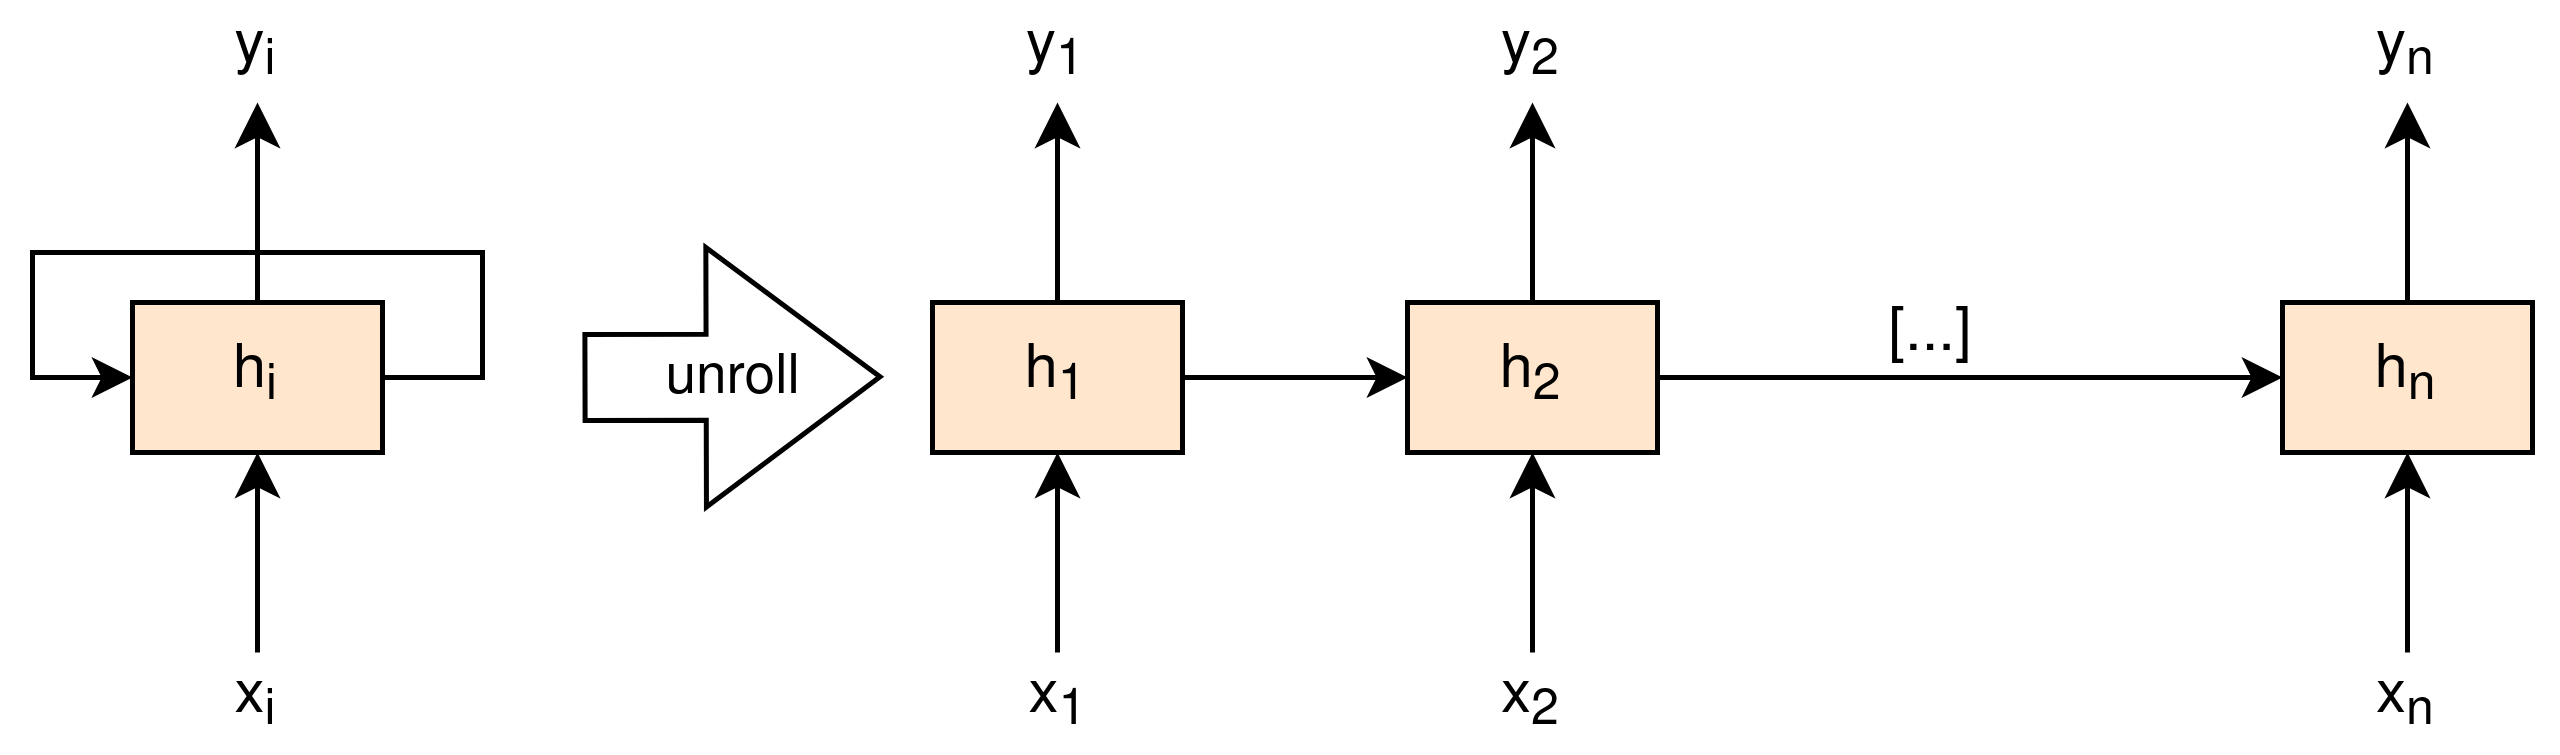
\includegraphics[width=0.7\linewidth]{img/RnnUnrolled}
        \caption[Unrolled structure of an RNN]{Structure of an RNN (left) and its unrolled version (right).
            $x_i$ are the inputs, $h_i$ are the hidden states and $y_i$ are the outputs.
            $n$ is the total number of tokens.
        }
        \label{fig:rnn-unrolled}
    \end{figure}

    % flow: description RNN structure
    On the left side you can see the RNN cell at a time step $i$.
    It receives the input token $x_i$ and the hidden state $h_{i-1}$ and produces the output $y_i$.
    It also updates the hidden state and passes the new hidden state $h_i$ back to the cell for the next time step.
    On the right, the unrolled version of the RNN reveals how the hidden states flow from one time step to the next.

    % flow: no parallelization
    Since the updated hidden state of the previous token is needed to calculate the next token, the outputs have to be calculated one after the other.
    This is the reason why the calculation within a RNN cannot be parallelized.

    % flow: bad long-range dependency detection
    Now, consider a sequence of length $n$ with a long-range dependency, for example between the first and the last token.
    Between them is a distance of length $\mathcal{O}(n)$ because the hidden state is updated for each of the $n - 2$ intervening tokens.
    At each update, the information of the first token or parts of it may be overwritten.
    Thus, the RNN is poor at detecting long-range dependencies.

    \subsection{Transformer architecture}\label{subsec:transformer-architecture}
    % flow: introduction to attention is all you need paper
    The 'Attention is all you need' paper~\cite{vaswani2017attention} marked the end of the RNN era with the previously mentioned drawbacks.
    The presented transformer architecture made it possible to parallelize training and better handle long-range dependencies.
    The novelty is not the use of attention mechanisms, but that it is built exclusively from them.
    Like RNNs, the transformer is originally designed for a sequence-to-sequence learning task, such as machine translation.

    \subsubsection{General flow through the transformer}
    % flow: figure transformer architecture
    \begin{figure}[btp]
        \centering
        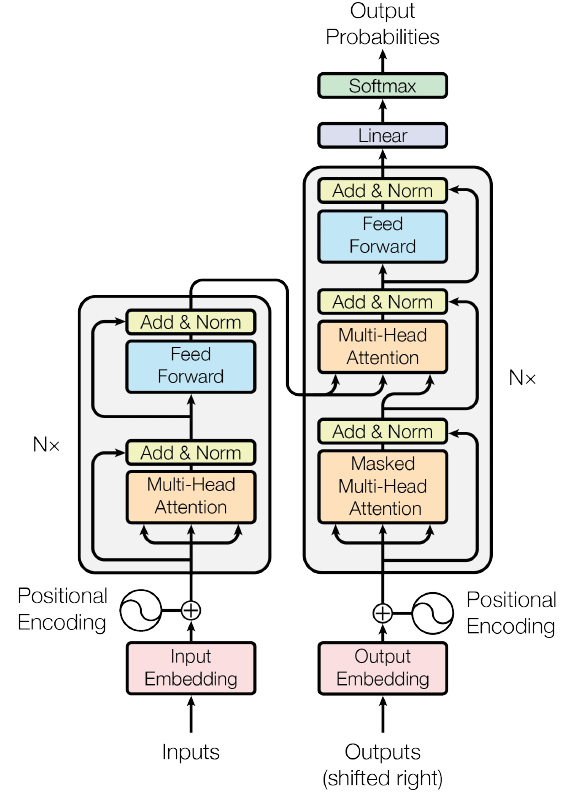
\includegraphics[width=0.75\linewidth]{img/TransformerModelArchitecture}
        \caption[Transformer architecture]{Transformer architecture consisting of stacked encoder cells (entire gray cell on the left) and stacked decoder cells (entire gray cell on the right).
        Only one encoder and one decoder cell are shown here.
        If there are several encoder and decoder cells, only the output of the last encoder cell is passed to the decoder cells as input (arrow from encoder to decoder cell).
        However, this output is passed to every decoder cell.
        'Norm' is the abbreviation for normalization layer.
        Figure is taken from~\cite{vaswani2017attention}}
        \label{fig:transformer-architecture}
    \end{figure}

    % flow: transformer architecture
    In figure~\ref{fig:transformer-architecture} the inner structure of a transformer is shown.
    We give an overview and explain the details step by step afterwards.
    The transformer takes sequences of length $n$ as input and outputs sequences of the same length.
    By padding the input with a special padding token [PAD], it can handle smaller input sequences.
    Part of the output is a special start-of-sequence [SOS] and a special end-of-sequence [EOS] token.
    The actual output lies in between of them and thus can be smaller than $n$.

    % flow: way through encoder structure
    First, the input tokens are passed through an embedding layer.
    Then, a positional encoding is added.
    The results are fed into stacked encoder cells.
    The output of the previous encoder cell is the input sequence of the next encoder cell.
    The purpose of the encoder cells is to generate a representation of the input sequence.

    % flow: way through decoder structure
    The right side of the figure represents the decoder part of the transformer, which is responsible for generating the output sequences.
    Here one has to distinguish between training and inference.

    % flow: figure transformer example
    \begin{figure}[btp]
        \centering
        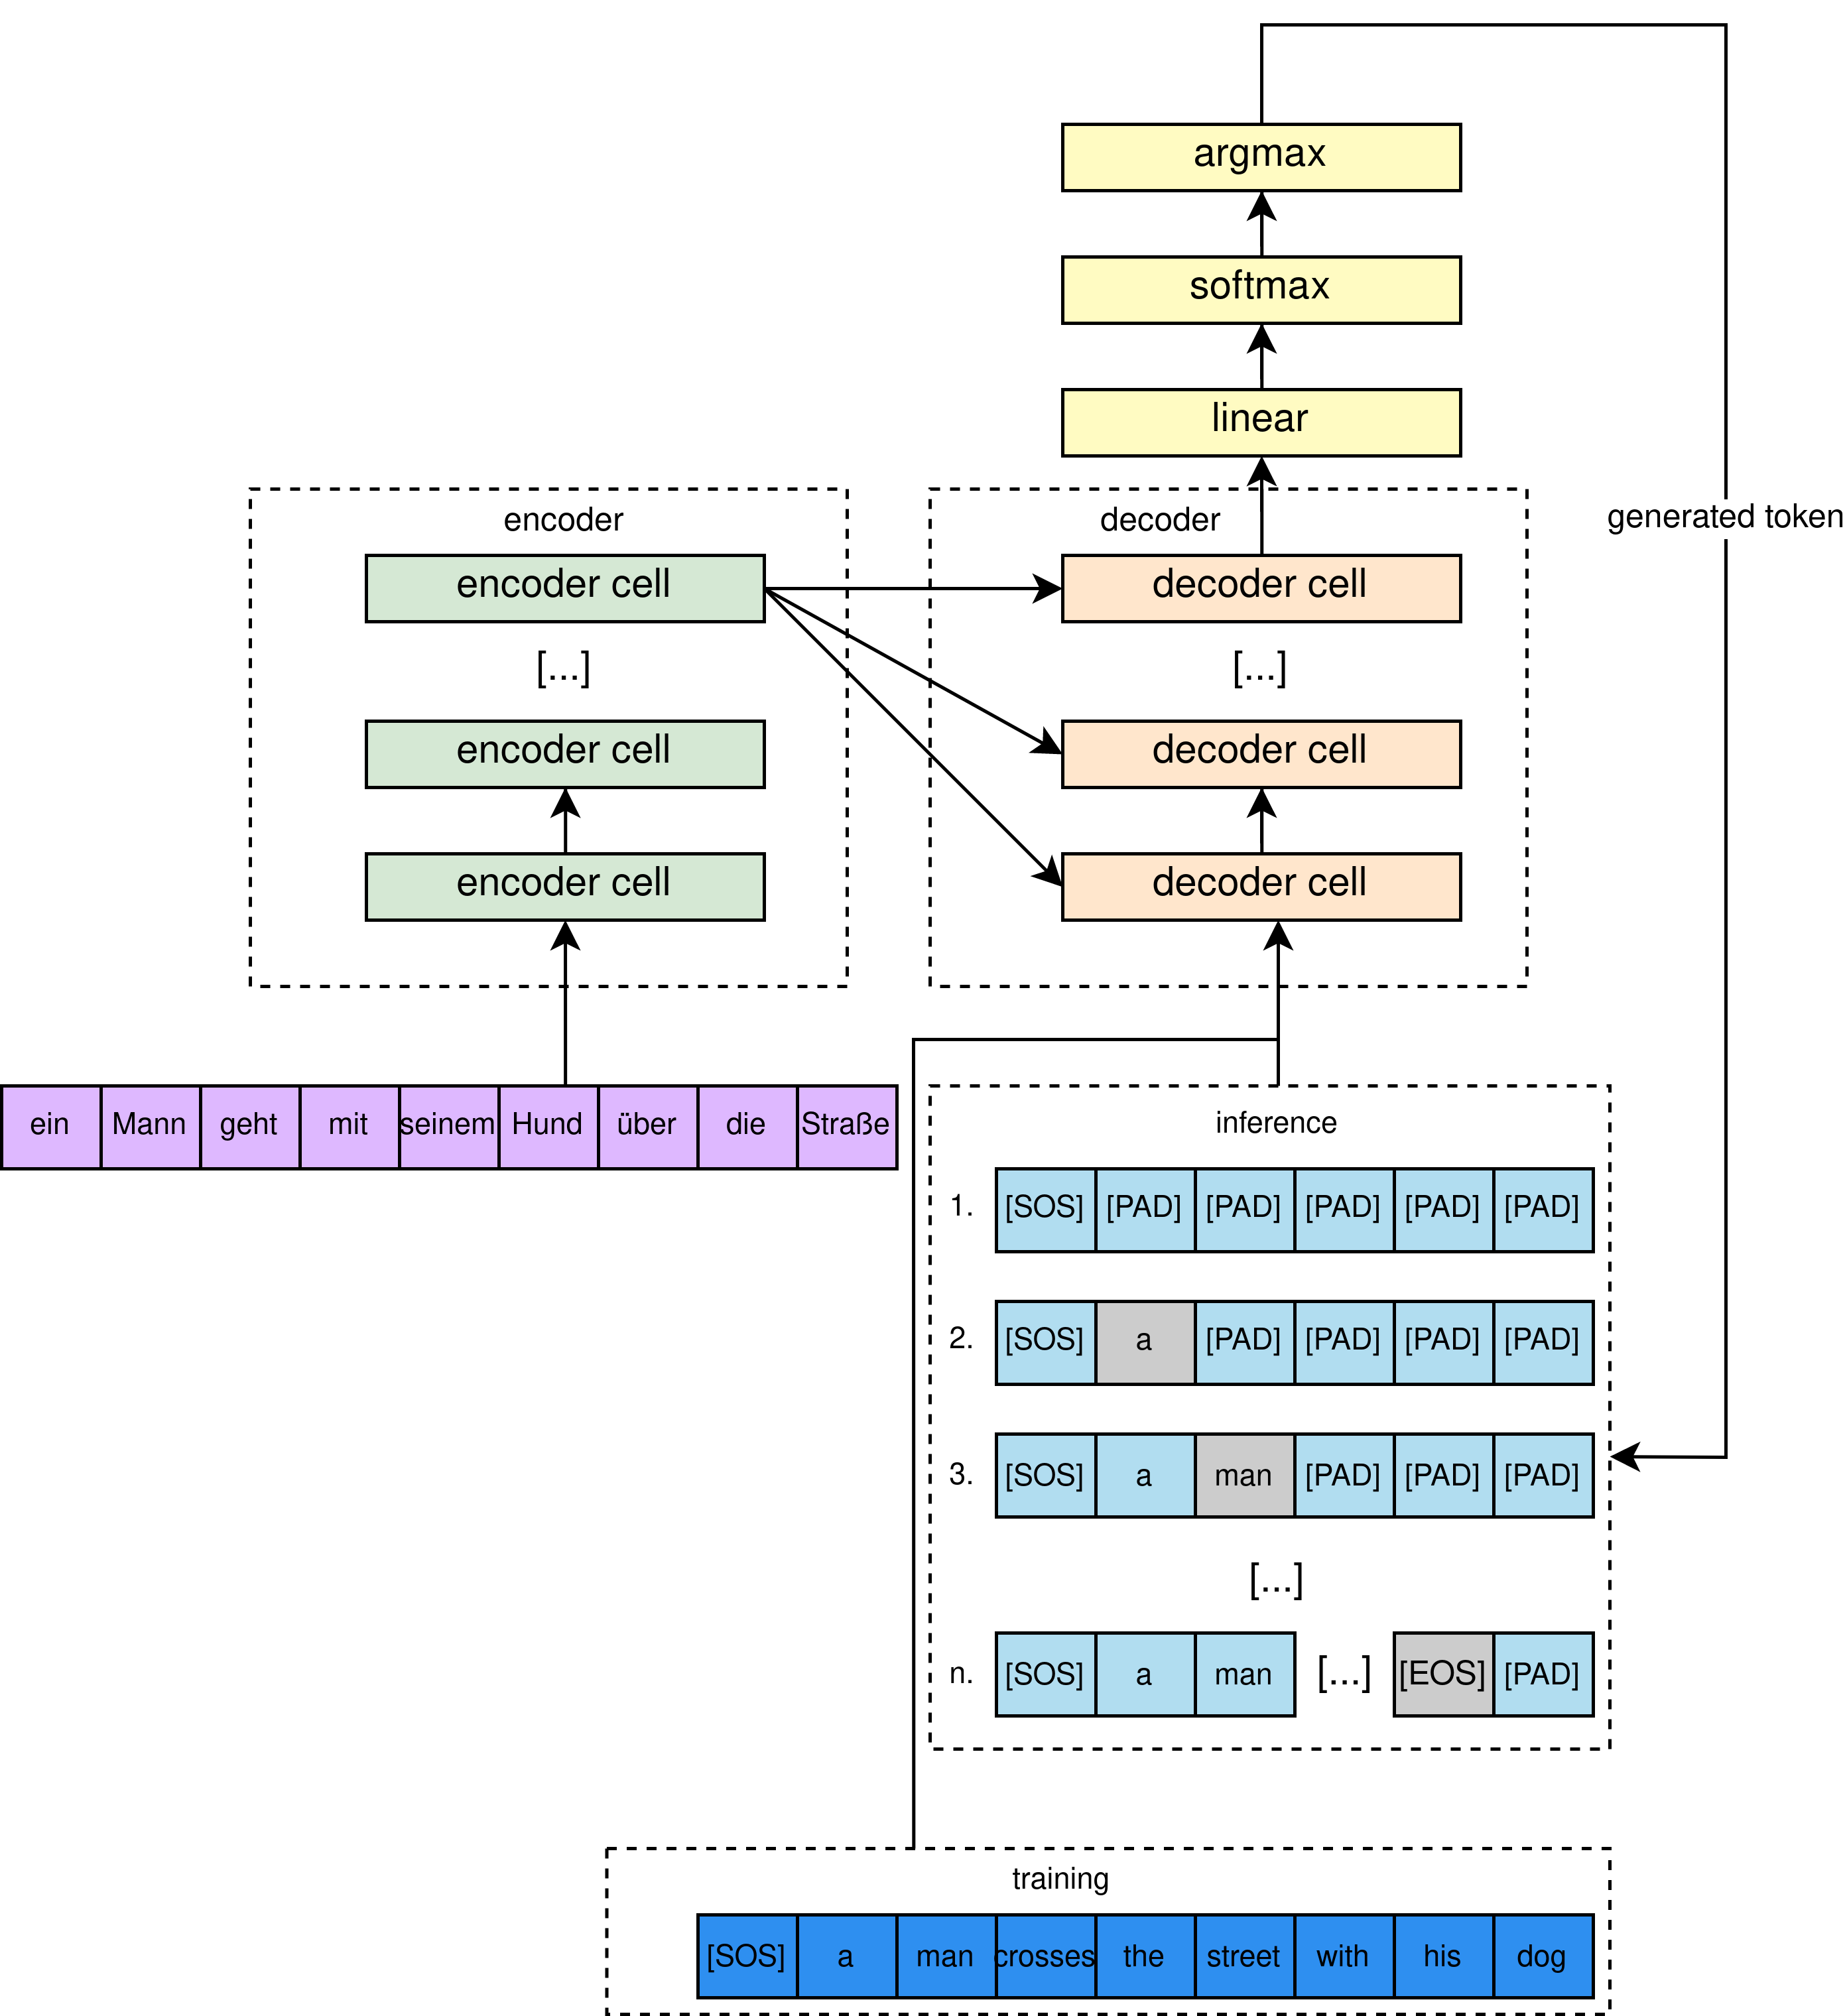
\includegraphics[width=\linewidth]{img/TransformerExample}
        \caption[Example inputs to the encoder and decoder cell]{
            Example of the inputs for the encoder and decoder cell at inference and training for translating the input sequence 'ein Mann geht mit seinem Hund über die Straße' into english.
            The left side of the figure shows how the purple input sequence is passed to the stack of encoder cells.
            The output of the last encoder cell is passed to all decoder cells as additional input.
            This is the case during both inference and training.
            During inference, the light blue token sequences are sequentially passed to the stack of decoder cells.
            The generated token is appended to the input sequence after the [SOS] sequence.
            It is highlighted in gray at each time step.
            At time step $n-1$ the [EOS] token is generated and appended to the input sequence for time step $n$.
            Now, the iteration stops.
            During training, the token sequence in dark blue is passed to the decoder.
        }
        \label{fig:transformer-example}
    \end{figure}

    % flow: decoder at inference time
    Figure~\ref{fig:transformer-example} shows an example of inputs for the decoder at inference and training time.
    During inference a list of generated tokens is maintained.
    At the beginning it contains only the [SOS] token.
    This list is padded up to length $n$ with [PAD] tokens and then passed to the decoder cells.
    As in the encoder part, this sequence is embedded and a positional encoding is added.
    Then it is passed through stacked decoder cells.
    Again, the output of the previous decoder cell is the input sequence of the next decoder cell.
    Each decoder cell receives the output sequence of the last encoder cell as additional input.
    All tokens of the output sequence of the last decoder cell are mapped to the vocabulary size using the same linear layer.
    The softmax is applied to each output to calculate probability distributions among the words of the vocabulary.
    The argmax of each distribution is taken to map it to a word of the vocabulary.
    In the first time step, the word produced by the first token is taken and appended to the list of generated tokens.
    More generally, at time step $t$ the word produced by the token at position $t$ is the next generated token.
    This process is repeated until the [EOS] token is generated.
    The inference can only be done sequentially because one needs the previously generated token to generate the next one.

    % flow: decoder at training time
    Since we know the label for a training example during training, we know the complete output sequence in advance.
    We shift this sequence by one position to the right and insert the [SOS] token at the first position.
    This sequence is passed through the decoder as in inference.
    Now, we pass each token of the resulting sequence to the linear layer and compute the softmax for each output.
    We take the argmax of each output and compare this sequence with the original label.
    Then the loss is computed and the weights are adjusted based on the gradients.
    During the calculations in the decoder cells, the tokens are prevented from seeing the tokens to their right, because these are the tokens that have not yet been generated during inference.
    Otherwise, they would just learn to copy them to the output.

    % flow: number of encoder and decoder cells
    In the original work, 6 encoder and 6 decoder cells were proposed.
    However, the number of cells is a hyperparameter and hast to be fitted to the actual problem.

    \subsubsection{Token embedding and positional encoding}
    % flow: embedding in the transformer
    Before the input is passed to the stack of encoder or decoder cells, it is embedded.
    This is only done once before the first cell and not before each cell.
    In the transformer, the embedding consists of two steps, token embedding and positional encoding.

    % flow: token embedding
    Token embedding is a quite common approach and not limited to transformers.
    The goal is to convert the sparse one-hot vectors of vocabulary words into smaller, dense vectors.
    Vectors with similar meanings should have a small distance between them.

    % flow: positional encoding
    The second part of the embedding is the positional encoding.
    While token embedding focuses only on the meaning of the word, positional encoding focuses where the word occurs in the sequence.
    RNNs receive the input token by token and can therefore store this information in the hidden state.
    On the other hand, transformers receive the entire input sequence at once and miss this information.
    The solution is to add positional encoding before passing the sequence to the encoder or decoder cells.
    This positional encoding depends only on the position of the word in the sequence and not on its meaning.
    In the following we show to approaches to calculate it.
    Both approaches produce similar results in performance~\cite{vaswani2017attention}.

    % flow: fixed functions
    The first is to use fixed functions that take the position as input and produce outputs of the same dimension as the token embedding.
    For example, if $d$ is the dimension of the token embedding, one could use the following function for each component $i$ of the $d$-dimensional token embedding:

    \begin{equation}
        \text{PositionalEmbedding}(p, i) = \sin\biggl(\frac{p}{100000^{i/d}}\biggr)\label{eq:pos-embed}
    \end{equation}


    where $p$ is the position of the word in the sequence.
    Thus, a sinusoidal wave of different length is used in each dimension.
    With such a fixed function, an already trained model can be extended to longer sequences without any changes.

    % flow: learned embeddings
    The second approach is to use a learnable variable of size $d$ for each position.
    The corresponding position variable is added to each input token.
    These variable are updated in the optimization step.
    This is a more generic approach because the transformer can model the positional encoding on its own.
    However, this cannot be extended to longer sequences without introducing and training new variables.

    \subsubsection{Encoder cell}
    % flow: stucture of an encoder cell
    Each encoder cell consists of two sections, the multi-head attention section and the feed-forward section.
    Both sections are wrapped by residual connections.
    When the input sequence $X$ is passed to the multi-head attention or the feed-forward section, the output is a sequence with the same length and dimension in both cases.
    This output is not treated as the final output, but added to the input sequence $X$.
    This is a common approach used in ResNets~\cite{he2015deep} to speed up training of very deep neural networks.
    Then, a layer normalization is performed.
    The computation of the multi-head attention section can be formulated as follows.
    \begin{equation}
        \text{LayerNormalization}(X + \text{MultiHeadAttention}(X))\label{eq:attention}
    \end{equation}
    The second section, the feed-forward section, computes the following:
    \begin{equation}
        \text{LayerNormalization}(X + \text{FeedForward}(X))\label{eq:feedforward}
    \end{equation}

    \subsubsection{Multi-Head Attention section}\label{subsubsec:multi-head-attention-section}
    % flow: row vector assumption
    \textit{In all equations in this and the following sections the vectors are assumed to be row vectors.}

    \bigskip

    % flow: single to multi head attention block
    The multi-head attention block consists of multiple attention heads.
    Within such an attention head, the scaled dot-product attention is calculated.
    We describe first how such an attention head is build and then how they are combined to a multi-head attention block.

    \paragraph{Scaled-dot product attention}
    % flow: multi-head attention
    We explain the scaled dot-product attention later in detail, but the key idea is to replace each token of the input sequence with a weighted average of all tokens.
    By assigning high and low weights to the token, the transformer can give different amounts of attention to the tokens.

    % flow: distance reduced
    Since each token can assign weights directly to every other token, the distances between them are reduced to $\mathcal{O}(1)$.

    % flow: figure example of attention
    \begin{figure}[btp]
        \centering
        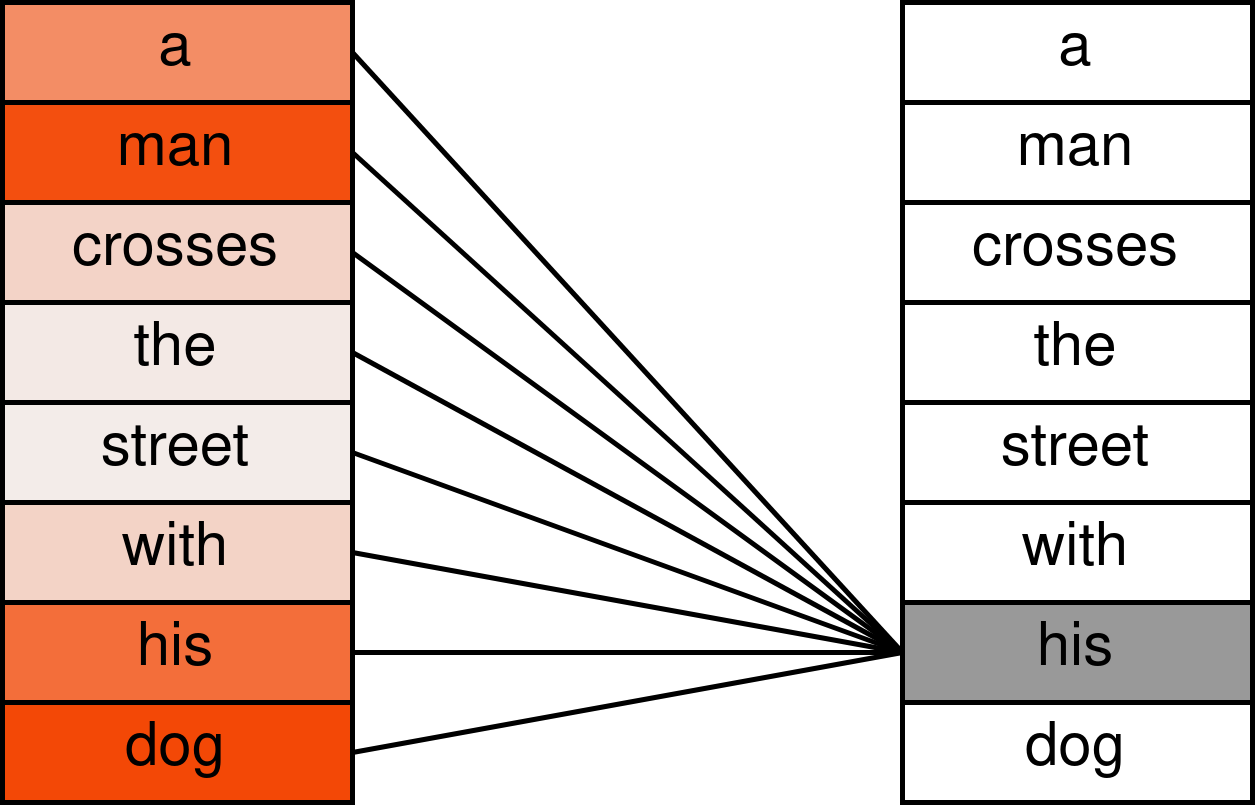
\includegraphics[width=0.5\textwidth]{img/TransformerAttentionExample}
        \caption[Example of attention inside the transformer]{Example of attention inside the transformer.
        The left sequence is the input sequence and the right sequence is the output sequence.
        Attention is only visualized for the word 'his' of the output sequence.
        The more colored the word is, the higher the attention weight of this word is.
        }
        \label{fig:transformer-attention-example}
    \end{figure}

    % flow: attention example
    In figure~\ref{fig:transformer-attention-example} an example of such an weighted average calculation is shown for a single token.
    The left part shows the input token sequence and the right part shows the output token sequence.
    The tokens are labeled with the actual words.
    For the output word 'his' the weights of the weighted average are visualized.
    The words 'a', 'man', 'dog' and the word 'his' itself have the highest weights.
    These are exactly the words needed to understand the meaning of the pronoun.

    % flow: first single exaple -> extend to entire sequence
    Now, we formulate this approach for a single token $x$ and explain afterwards how to extend the calculation to the entire input.
    Mathematically, the token $x$ can be thought of as a vector.

    % flow: weight matrices
    In the transformer there are three weight matrices that are updated during optimization:
    The query weight matrix $W^Q$, the key weight matrix $W^K$ and the value weight matrix $W^V$.
    By multiplying $x$ with each of these weight matrices a query vector $q_x$, a key vector $k_x$ and a value vector $v_x$ are derived:

    \begin{gather}
        q_x = x * W^Q  \label{eq:query-vec} \\
        k_x = x * W^K  \label{eq:key-vec} \\
        v_x = x * W^V  \label{eq:value-vec}
    \end{gather}

    % flow: calculate attention
    The query, key and value vectors are calculated for every token.
    To calculate the weights for the weighted average, the query vector $q_x$ of $x$ is sent to each token $x'$ of the input sequence and multiplied by its key vectors $k_{x'}$.
    These weights are scaled by $1 / \sqrt {d_k}$, where $d_k$ is the dimension of the keys.
    Last, a softmax is applied to the weights and the weighted average is calculated.
    Excluding the softmax calculation, the above can be formulated as follows:

    \begin{equation}
        \text{ScaledDotProductAttention}(x) = \sum_{x'} (\frac{1}{\sqrt {d_k}} q_x * k_{x'}^T) v_{x'}\label{eq:scaled-dot-vector}
    \end{equation}

    % flow: extension to matrices
    Instead of calculating this sequentially for every token, we can formulate it using matrices and do the calculation all at once.
    We put the input sequence together into a matrix $X$, where the first row is the first token, the second token is the second row and so on.
    Then we can perform calculations similar to those in equations~\ref{eq:query-vec},~\ref{eq:key-vec} and~\ref{eq:value-vec} to obtain the query, key and value matrices $Q$, $K$ and $V$:

    \begin{gather}
        Q = X * W^Q \label{eq:query-mat} \\
        K = X * W^K \label{eq:key-mat} \\
        V = X * W^V \label{eq:value-mat}
    \end{gather}

    % flow: weight-sharing
    The matrices $W^Q$, $W^K$ and $W^V$ are the same as in equations~\ref{eq:query-vec},~\ref{eq:key-vec} and~\ref{eq:value-vec}.
    Therefore, the number of parameters of the transformer encoder and decoder cells does not depend on the length of the input sequence.

    % flow: matrix scaled dot-product
    Similar to equation~\ref{eq:scaled-dot-vector} we can calculate the scaled dot-product attention, this time with the softmax calculation included:

    \begin{equation}
        \text{ScaledDotProductAttention}(X) = \text{softmax}(\frac{QK^T}{\sqrt {d_k}})V \label{eq:scaled-dot-mat}
    \end{equation}

    % flow: summation in matrix multiplication
    The softmax calculation returns a $n\times d_k$ matrix.
    We retrieved just one row of it in equation~\ref{eq:scaled-dot-vector} and had to model the summation explicitly.
    Here, another matrix multiplication with $V$ is used to scale and sum up the value vectors.

    % flow: figure scaled dot-product attention and mulit-head attention
    \begin{figure}[btp]
        \centering
        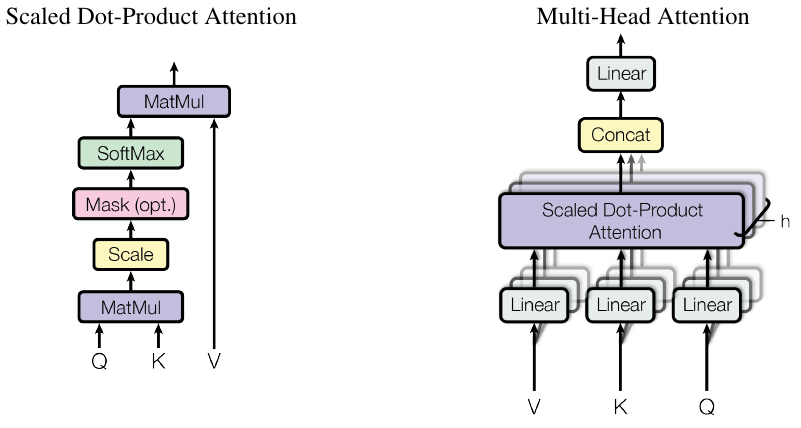
\includegraphics[width=0.75\linewidth]{img/TransfomerAttentionAndMultihead}
        \caption[Scaled dot-product attention and multi-head attention]{The left side shows how the scaled dot-production attention is calculated from the query matrix $Q$, the key matrix $K$ and value matrix $V$.
        MatMul stands for matrix multiplication.
        The optional mask block is only used in the decoder.
        The right side shows how $h$ different attention heads are combined to a multi-head attention head, where $h$ is the number of the attention heads.
        Figure is from~\cite{vaswani2017attention}}
        \label{fig:transformer-attention-calculation}
    \end{figure}

    % flow: mask block in figure optinally
    This calculation is visualized on the left side of figure~\ref{fig:transformer-attention-calculation}.
    An optional mask block is already included which we will explain later in the decoder part.

    \paragraph{Combination of different attention heads}
    % flow: multi-head attention
    On the right side of figure~\ref{fig:transformer-attention-calculation} the combination of $h$ different attention heads is illustrated.
    $Q$, $K$ and $V$ are calculated as described in equations~\ref{eq:query-mat},~\ref{eq:key-mat} and~\ref{eq:value-mat}.
    For each attention head $i$ they are multiplied by the parameter matrices $W^Q_i$, $W^K_i$ and $W^V_i$ to obtain the the query, key and value matrices $Q^i$, $K^i$ and $V^i$:

    \begin{gather}
        Q^i = Q * W^Q_i \\
        K^i = K * W^K_i \\
        V^i = V * W^V_i
    \end{gather}

    % flow: project back to input
    Now, the scaled dot-product attention is calculated with equation~\ref{eq:scaled-dot-mat} using the matrices $Q^i$, $K^i$ and $V^i$.
    The resulting matrices are concatenated row by row and linearly projected back to the dimension of the input sequence, as shown in the upper right of figure~\ref{fig:transformer-attention-calculation}.

    % flow: why multi-head attention
    In~\cite{vaswani2017attention} there have been experiments made to compare a single attention head with large dimensions to a multi-head approach with small dimensions.
    To obtain similar computational costs, the dimension of the single head was set to the sum of the dimensions of the heads of the multi-head attention head.
    The multi-head approach performed better than the single head and thus was used in the transformer architecture.

    \subsubsection{Feed-Forward section}\label{subsubsec:feed-forward-section}
    The feed-forward section consists of two fully-connected layers with a ReLU activation in between.
    The same fully-connected layer is applied to each token of the input sequence.
    So, for each token $x$ of the input sequence $X$ the feed-forward is calculated:

    \begin{equation}
        \text{FeedForward}(x) = \max(0, x * W_1 + b_1)W_2 + b_2\label{eq:feed-forward}
    \end{equation}

    \subsubsection{Decoder cell}
    % flow: recap decoder cell
    Now, we return to figure~\ref{fig:transformer-architecture} to describe the decoder cell in detail.
    The input of the decoder cell is a sequence of tokens that are embedded with the two step approach as in the encoder.
    The output of the decoder is also a sequence with the same dimension as the input.
    The output of the last decoder cell is passed to a linear layer to project it to the vocabulary size.
    A softmax calculation followed by an argmax calculation is used to choose a word of the vocabulary.
    During inference, the word corresponding to the current time step is selected whereas during training all words are considered in the loss calculation.

    % flow: sections of decoder cell
    Let us take a look inside the decoder cell.
    We can divide it into three sections.
    The first section contains a masked multi-head attention block.
    The second sections contains a normal multi-head attention bock.
    Here, the output of the last encoder flows in.
    The third section contains a feed-forward network.
    As in the encoder each of these sections are wrapped by residual connections and followed by a layer normalization.
    We explain these sections in this order.

    % flow: masked multi-head attention section
    During training, the entire label sequence is passed to the transformer.
    We have already mentioned that inside the decoder it is prevented that tokens can see tokens to their right.
    This is the purpose of the mask.
    In the left part of figure~\ref{fig:transformer-attention-calculation} you can see how the mask is inserted in the scaled dot-product attention.
    Thus equation~\ref{eq:scaled-dot-mat} changes to:

    \begin{equation}
        \text{ScaledDotProductAttention}(X) = \text{softmax}(\text{mask}(\frac{QK^T}{\sqrt {d_k}}))V\label{eq:scaled-dot-mask}
    \end{equation}

    The mask operation sets values that correspond to weights of tokens to the right to $- \inf$.
    The softmax calculation transforms these values to $0$, such that they are excluded from the weighted average.
    Only in this multi-head attention section the mask is applied.
    The other ones remain as previously described.

    % flow: mutli-head attention section
    The second section of the decoder cell is similar to the multi-head attention section of the encoder.
    Only the query and key matrix $Q$ and $K$ are derived from the output sequence of the last encoder cell.
    The value matrix $V$ is derived from the output sequence of the previous decoder cell as usual.
    With $X$ as the output of the previous decoder cell and $Y$ as the output of the last encoder cell, the equations~\ref{eq:query-mat},~\ref{eq:key-mat} and~\ref{eq:value-mat} change to:

    \begin{gather}
        Q = Y * W^Q \\
        K = Y * W^K \\
        V = X * W^V
    \end{gather}

    % flow: feed-forward section
    The feed-forward section is identical to the one described in~\ref{subsubsec:feed-forward-section}.

    \subsection{Modifying the Transformer architecture for classification}\label{subsec:using-transformers-for-classification}
    % flow: tranformer for generation image
    The previously described transformer architecture was designed for sequence-to-sequence learning tasks.
    However, we show how it can be modified to use transformers for classification.
    For this purpose, we use BERT as an example.
    Since no output sequences need to be generated, only the encoder cells of the transformer architecture are used in BERT\@.

    % flow: BERT intro
    BERT stands for \textbf{B}idirectional \textbf{E}ncoder \textbf{R}epresentations from \textbf{T}ransformers and is one prominent application of a transformer in NLP\@.
    Nowadays it is an established basis for transfer learning tasks for many NLP applications.

    % flow: BERT architecture
    In figure~\ref{fig:bertArchitecture} a model of BERTs architecture can be seen.
    The input of BERT consists of up to two input sentences.
    This may be useful if the first sentence is a question and the second one is a paragraph containing the answer, and the task of the model is to predict the beginning and end of the answer.
    BERT inserts an extra classification token [CLS] before the sentences and separates them with a separation token [SEP].
    This entire sequence is now passed through stacked transformer encoders.

    % flow: figure BERT architecture
    \begin{figure}[btp]
        \centering
        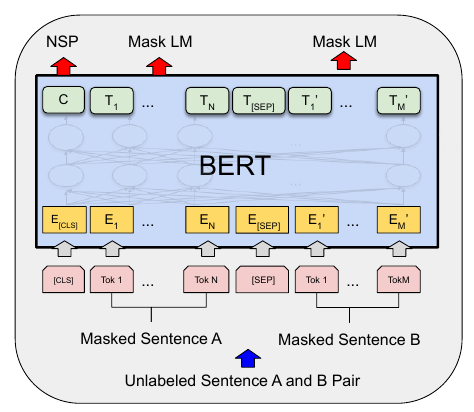
\includegraphics[width=0.5\linewidth]{img/BertArchitecture}
        \caption[BERT Archtitecture]{The architecture of the BERT model. Two unlabeled sentences A and B are passed to a transformer.
        During pre-training, the output of the classification token is used for next sentence prediction (NSP).
        This token is used for fine-tuning the BERT model for classification tasks.
        The rest of the transformed sequence is used for the masked language model (mask LM) during pre-training and fine-tuned to the task at hand.
        Figure is taken from~\cite{devlin2019bert}}
        \label{fig:bertArchitecture}
    \end{figure}

    % flow: BERT pre-training
    BERT was pre-trained on two different tasks.
    The first one is next-sentence prediction.
    As input, the model receives two sentences and must predict whether the second sentence is a correct continuation of the first one.
    The classification is done with a feed-forward network which receives only the output of the [CLS] token.
    The second one is masked language model.
    Here, 15\% of the input tokens are masked replacing them with either a [MASK] token or by a random word, and the model's task is to recover the masked words.
    For both tasks, it has been trained on huge datasets.

    % flow: BERT fine-tuning
    To fine-tune BERT, only the inputs of the respective task have to be fed into BERT and the required outputs have to be processed.
    All parameters are updated during fine-tuning.

    % flow: BERT performance
    BERT lead to several improvements in NLP\@.
    For example, a score of 80.5\% was achieved on the General Language Understanding Evaluation (GLUE) benchmark, which is 7.7\% above the previous high score.

    % flow: summary classification with transformers and transition to image classification
    So, to use transformers for classification we add a [CLS] token in front of the sequence and feed this through stacked encoder cells.
    Then, we use only the output of the [CLS] token to classify the example with a feed-forward network.
    In the next chapter, we show how to use this approach for image classification.

    \clearpage

% ==============================


    \section{Transformers for image classification}\label{sec:transformers-for-image-classification}
    % flow: intro image transformer
    In the last chapter we presented the transformer architecture and how it is modified for classification.
    It is widely used in NLP and has been very successful.
    There is also a lot of research applying the concepts to image processing in hopes of achieving equally good results.
    In this chapter, we explain how to use transformers for image classification.

    \subsection{Detecting long-range dependencies with CNNs}
    % flow: recap distances in RNN and transformer
    In chapter~\ref{sec:transformers-in-nlp} we explained that transformers are superior to RNNs because they reduced the distance between tokens from $\mathcal{O}(n)$ to $\mathcal{O}(1)$.
    Thus, long-range dependencies can be better detected with transformers.
    Let us now analyse the distance in CNNs.

    % flow: stacked convolution layers
    To classify images with convolutions, multiple convolutional layers are stacked.
    The idea is that the first layers detect edges and corners and the following layers can combine them into increasingly complex features.
    Low-level features can be detected very easily, but the more complex the features become, the more convolutions are needed to detect them.
    The reason for this is that one convolution can only look for one feature.

    % flow: figure convolution kernel
    \begin{figure}[hbtp]
        \centering
        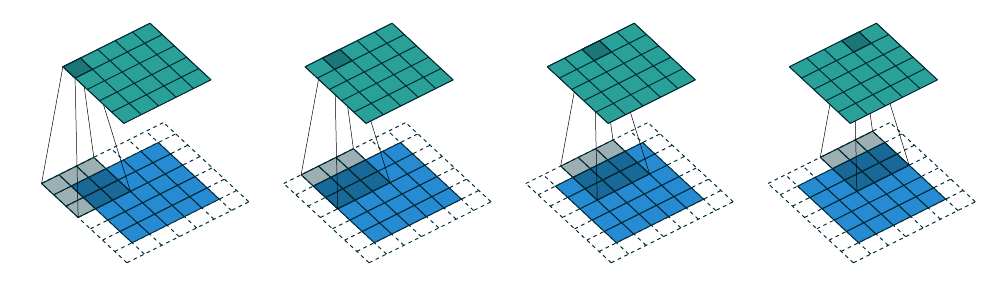
\includegraphics[width=0.95\linewidth]{img/ConvolutionKernel}
        \caption[Convolution Kernel]{
            The blue squares are the input padded with the dashed squares.
            The green square are the output.
            The highlighted regions correspond to the $3 \times 3$-kernel of the convolution and its output.
            Figure is taken from~\cite{dumoulin2018guide}}
        \label{fig:convolution-kernel}
    \end{figure}

    % flow: description convolution kernel
    In figure~\ref{fig:convolution-kernel} an example convolution is shown.
    Here, a $3 \times 3$-kernel with a stride of $1$ and a padding of $1$ is used.

    % flow: distance in convolutions
    Consider an input of size $n \times n$ and a convolution with kernel size $k \times k$, a stride of size $k$ and no padding.
    Focusing only on one dimension, we see that the $n$ inputs are divided into $n/k$ blocks of size $k$.
    Each of these blocks is reduced to an output of size 1.
    The next convolution layer then processes the sequence of length $n/k$ in the same way.
    So we see that $\mathcal{O}(\log_k (n))$ convolutional layers are needed until the rightmost and leftmost inputs are in the same block.
    We have to double this bound, if we take the second dimension back into consideration, because this distance occurs in both dimensions.
    However, in big-O notation it remains the same.
    Padding only adds blocks to the calculation at the edges and therefore has no effect on this bound.
    If the stride is lower than $k$, the number of blocks that are generated is even higher than $n/k$.
    Therefore, we can give $\mathcal{O}(\log_k (n))$ as a lower bound for the distance in convolutions.

    % flow: transformers better
    This result is better compared to RNNs.
    However, the constant distance with transformers seems promising for images.
    In the following sections, we describe different approaches to achieve this goal and evaluate their performance in chapter~\ref{sec:evaluation-of-the-transformers-for-image-classification}.

    \subsection{Naive approach to use transformer for image classification}\label{subsec:naive-transformer}
    % flow: description naive transformer
    To use transformers for image classification one has to convert the input image into a sequence of tokens.
    The naive approach is to flatten the pixels of the image and treat each pixel as a token.
    Sine the image should be classified, the classification approach of BERT is used as shown in section~\ref{subsec:using-transformers-for-classification}.
    Again, a [CLS] is token is inserted at the front of the sequence.
    These tokens are embedded and passed to the normal transformer encoder as described in section~\ref{subsec:transformer-architecture}.

    % flow: computational complexity
    In each encoder cell of the transformer, a weighted average of all tokens is calculated for all tokens.
    Therefore, the computational complexity of this model is $\mathcal{O}(Ln^2)$, where $L$ is the number of encoder cells and $n$ is the number of pixels.
    In image processing, an encoder cell is also referred to as a transformer layer, as this terminology has more in common with the convolutional layers used in CNNs.
    Especially for high-resolution images, the computational cost becomes extremely expensive, making it impractical for inference and training.

    \subsection{Pure attention based transformers for image classification}
    % flow: intro pure attenton based transformers
    To overcome the complexity of the naive transformer the following models where introduced.

    \subsubsection{Vision Transformer}\label{subsubsec:vision-transformer}
    % flow: vision transformer
    The first and most famous approach is presented in the paper 'An image is worth 16x16 words'~\cite{dosovitskiy2021image}.
    The featured Vision Transformer is very similar to the naive approach.
    The only difference is that the image is split into 16x16 patches of the same size.
    The patches are embedded and passed to stacked transformer layers.
    Also, classification is performed using a classification token.
    This is illustrated in figure~\ref{fig:visionTransformerArchitecture}.

    % flow: reduction of complexity
    This reduces the theoretical complexity of each transformer layer from $\mathcal{O}(n^2)$ to $\mathcal{O}(1)$, because the number of patches no longer depends on the input size $n$.
    Nevertheless, the computational work is not negligible in practice.

    % flow: figure vision transformer architecture
    \begin{figure}[btp]
        \centering
        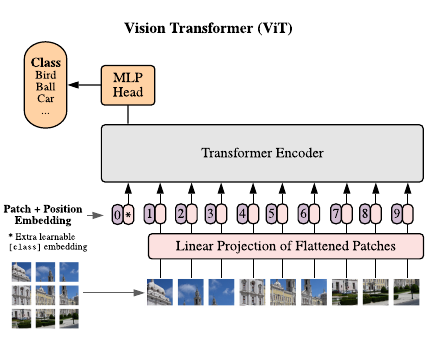
\includegraphics[width=0.55\linewidth]{img/VisionTransformerArchitecture}
        \caption[Vision Transformer Architecture]{Architecture of the vision transformer.
        On the left the input image and its division into patches is shown.
        The patches are flattened and passed to the 'linear projection of flattened patches' block that is identical to the token embedding.
        To the output of this the position encoding is added and passed to the transformer encoder that consists of multiple encoder cells.
        Only the output of the [class] embedding, which is the [CLS] token in our terminology, is passed to the MLP head.
        'MLP head' stands for multi layer perceptron and is a feed-forward network to make the final classification.
        Figure is taken from~\cite{dosovitskiy2021image}}
        \label{fig:visionTransformerArchitecture}
    \end{figure}

    \subsubsection{Dynamic Vision Transformer}\label{subsubsec:dynamic-vision-transformer}
    % flow: dynamic vision transformer
    The paper 'Not all images are worth 16x16 words' criticizes, that the empirically choice of the vision transformer to use 16x16 patches is not suitable for all images.
    It has been observed that there are many easy images for which already a small number of patches is sufficient.
    In addition to this, there exist hard images that need finer representations than 16x16.
    The presented Dynamic Vision Transformer uses a multiple Vision Transformers with increasing number of tokens.
    The image is passed through the transformers in order of increasing token count until the output is sufficiently confident.
    In this process the transformer reuses learned representations and relationships.
    The process is visualized in~\ref{fig:dynamic-vision-transformer}.

    % flow: figure dynamic vision transformer
    \begin{figure}[btp]
        \centering
        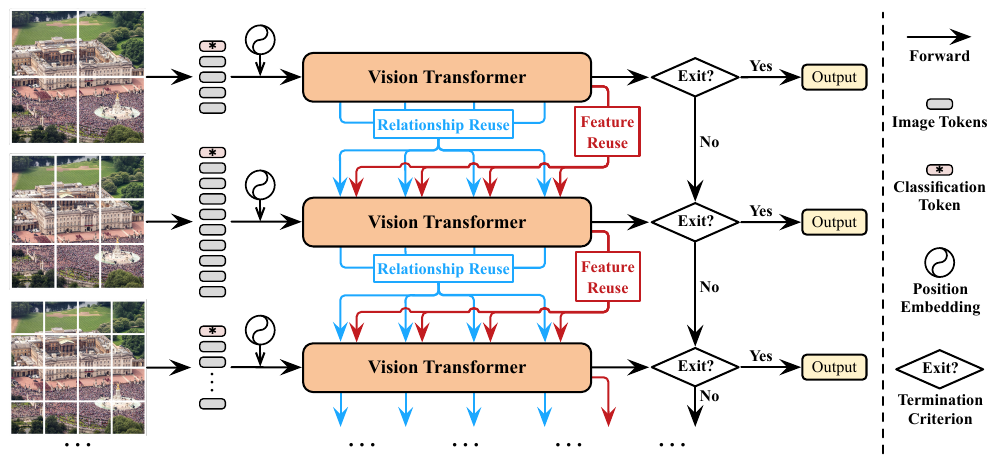
\includegraphics[width=0.85\linewidth]{img/DynamicVisionTransformer}
        \caption[Dynamic Vision Transformer]{
            Illustration of a dynamic vision transformer.
            The image is passed to an vision transformer with a rough resolution.
            Either the vision transformer is confident enough or the image is passed to the next vision transformer with finer resolution.
            This process is repeated until the image is classified or the last vision transformer is reached.
            In the latter case, the output of this transformer is used.
            Image is taken from~\cite{wang2021images}}.
        \label{fig:dynamic-vision-transformer}
    \end{figure}

    \subsubsection{Image Transformer}\label{subsubsec:image-transformer}
    % flow: intro image transformer
    Another solution, the Image Transformer, is presented in~\cite{parmar2018image}.
    Here, the attention mechanism is slightly modified by adding local restrictions to it.
    The Image Transformer is a model for image generation which is covered later in section~\ref{subsec:image-generation}.
    However, its modification of the attention mechanism can be also used for image classification.

    % flow: local restricted attention.
    The image is divided into non-overlapping query bocks.
    Each query block has a memory block associated with it.
    For each token of a query block, attention is restricted to the memory block of this query block.
    A 1D and a 2D method are proposed to select the blocks.
    Both are visualized in figure~\ref{fig:image-transformer-attention}.
    While the 1D solution is easier to implement, the 2D approach performs slightly better.
    One explanation is, that in the 1D approach more pixels from the far left and right are taken into consideration.
    The 2D approach, on the other hand, provides a good balance between the left and right pixels and the top and bottom pixels.

    % flow: complexity reduction
    The complexity is reduced from $\mathcal{O}(Ln^2)$ to $\mathcal{O}(Lmn)$, where $L$ is the number of transformer layers, $n$ is the number of pixels and $m$ is the size of the memory block, with $m < n$.

    % flow: figure image transformer
    \begin{figure}[btp]
        \centering
        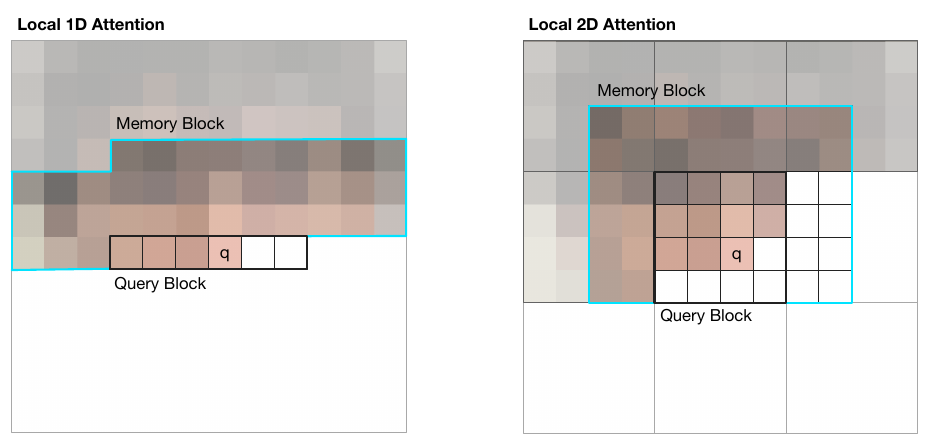
\includegraphics[width=0.65\linewidth]{img/ImageTransformerAttention}
        \caption[Local attention of the Image Transformer]{
            Local 1D attention on the left and local 2D attention on the right.
            In local 1D attention, the pixels are flattened and this sequence is divided into query blocks.
            For each query block, the $m$ pixels before are chosen as the memory block, where $m$ is the size of the memory block.

            For local 2D attention the query blocks are chosen as rectangular regions.
            For the memory blocks, these regions are expanded leftward and upward until $m$ pixels are reached.
            Figures are taken from~\cite{parmar2018image}}
        \label{fig:image-transformer-attention}
    \end{figure}

    \subsection{Hybrid Approaches}\label{subsec:hybrid-approaches}
    % flow: intro cnns
    Before transformers, CNNs were the dominant approach for image classification.
    Now, we focus on some hybrid approaches that combine the strengths of both.
    Therefore, CNNs are used to extract low-level features and transformers are used for adding global context.
    There is a variety of such models and we present only subset of them.

    \subsubsection{Visual Transformer}
    % flow: figure architecture visual transformer
    \begin{figure}[btp]
        \centering
        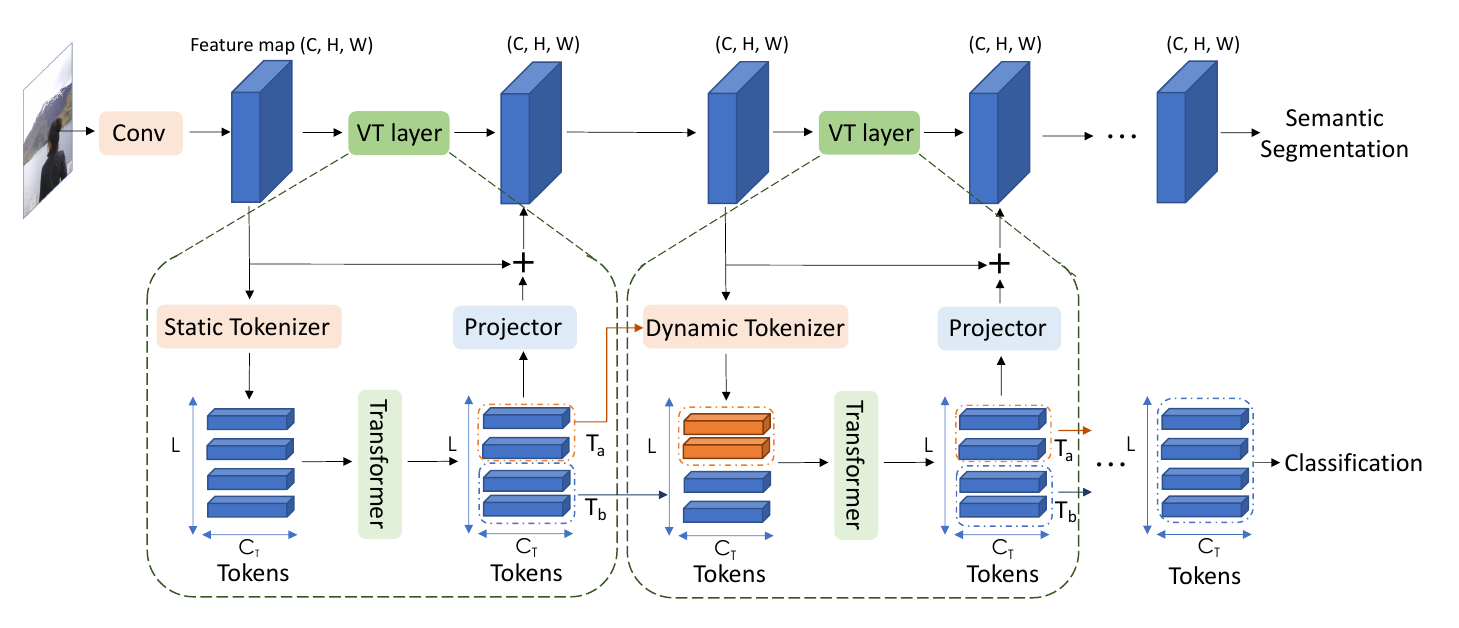
\includegraphics[width=\linewidth]{img/VisualTransformerArchitecture}
        \caption[Architecure Visual Transformer]{
            Architecture of the visual transformer.
            Two visual transformer bocks are shown surrounded by the dotted lines.
            In the left block a static tokenizer is used and in the right a dynamic tokenizer is used.
            Figure is taken from~\cite{wu2020visualV3}}
        \label{fig:visual-transformer-architecture}
    \end{figure}

    % flow: architecture visual transformer
    In figure~\ref{fig:visual-transformer-architecture} the architecture of the 'Visual Transformer'~\cite{wu2020visualV3} is shown.
    First, a feature map is generated with convolutions.
    These features are then processed by stacked visual transformers blocks.
    Such a block consists of a tokenizer, a transformer and a projector.
    The tokenizer uses convolutions to extract some features from the feature map.
    Now, the transformer adds some global context to the features, and the projector maps them back to the original feature map.
    Both use attention mechanisms.

    % flow: static and dynamic tokenizer
    In the first visual transformer block a static tokenizer is used.
    It extracts a fixed number of features from the feature map.
    In all subsequent visual transformer blocks dynamic tokenizers are used which extract a variable number of features.

    % flow: difference classification and semantic segmentation
    For classification tasks the output of the transformer inside the last visual transformer block before the back projection to the feature map is used.
    For semantic segmentation the output after the back projection is used.

    \subsubsection{Convolutional Neural Networks meet Vision Transformers}
    % flow: intro cmt
    Another approach is presented in the paper 'Convolutional Neural Networks meet Vision Transformers'~\cite{guo2021cmt}.
    Here, modified transformer layers are inserted into a traditional CNN\@.
    This increases the accuracy and reduces the computational cost.

    % flow: figure cmt architecture
    \begin{figure}[btp]
        \centering
        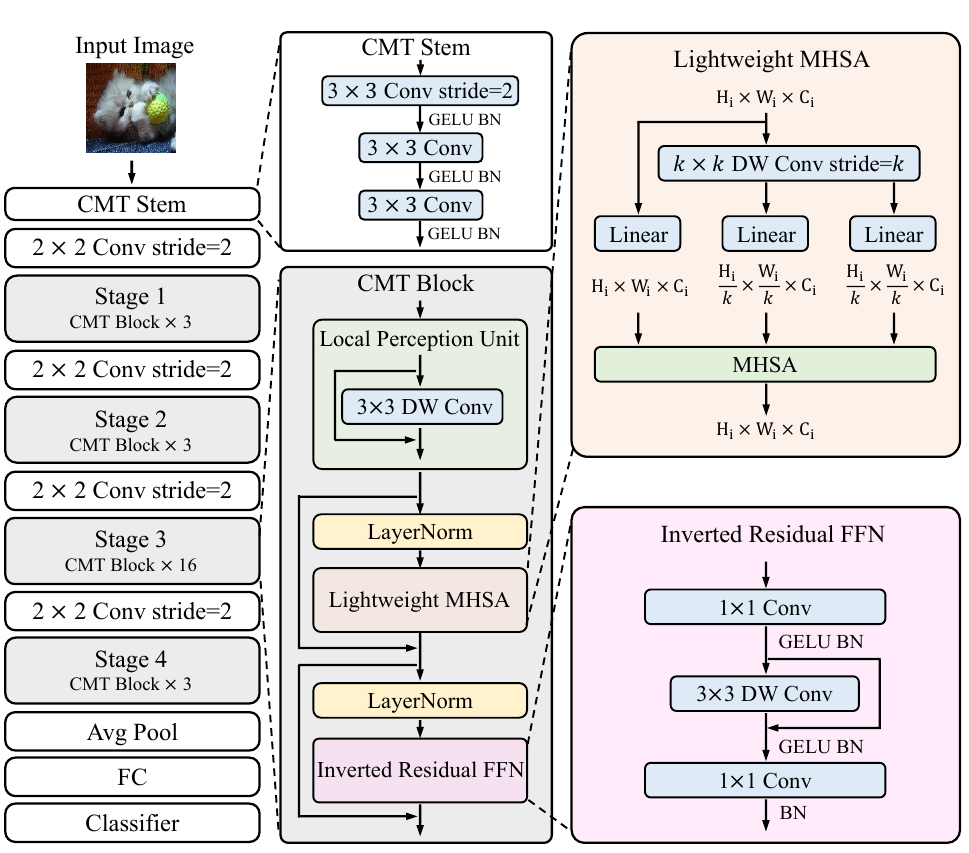
\includegraphics[width=0.7\linewidth]{img/CmtArchitecture}
        \caption[CMT Architecture]{CMT Architecture.
        CMT stands for CNNs meet transformers.
        A CTM Stem in the beginning and stacked CMT blocks are inserted between convolutions to improve the model.
        The CTM Stem consists of three stacked convolutions.
        CMT blocks consist of local perception units, lightweight multi head self attention (MHSA) and inverted residual feed forward networks (FFN).
        'DW Conv' stands for depth-wise convolution.
        'Avg Pool' is a average pooling layer and 'FC' is a fully-connected layer.
        Figure is taken from~\cite{guo2021cmt}}
        \label{fig:cmt-architecture}
    \end{figure}

    % flow: overall architecture
    Let us regard the architecture which is shown in figure~\ref{fig:cmt-architecture}.
    In the CMT Stem at the beginning, three stacked convolutions are used instead of splitting the image into patches as in the Vision Transformer.
    This is followed by alternating convolutions and CMT blocks.
    Finally, the average of the features is computed and passed through a feed forward network to a classification head.

    % flow: CMT block
    A CMT block consists of a local perception unit, a lightweight MultiHeadSelfAttention unit and an inverted residual feed forward network.
    The local perception unit is a depth-wise convolution enclosed by a residual connection.
    In the lightweight MultiHeadSelfAttention unit the dimensions of the key and value matrices are reduced, also by depth-wise convolutions.
    The inverted residual feed forward network uses a combination of normal convolutions and depth-wise convolutions to first increase the dimension by a constant factor and then reduce it back to its original dimension.

    \subsubsection{Glance-and-Gaze Transformer}
    % flow: glance-and-gaze transformer
    A different approach is used in the 'Glance-and-Gaze Transformer'~\cite{yu2021glanceandgaze}.
    This model is build an special glance-and-gaze transformer blocks.
    Such a block has two different branches, one glance branch that uses transformers to detect global dependencies and one gaze branch that uses convolutions to detect local features.
    At the end of each block, the results are combined.

    % flow: borth branches are useful
    Experiments have shown that neither branch can be omitted without drastically reducing performance.
    The Glance-and-Gaze Transformer achieved better accuracy results than the original Vision Transformer with less computational effort.

    \subsubsection{Teacher-student strategy specific to transformers}
    % flow: distillation token
    A completely different approach to improve transformers by using CNNs is presented in~\cite{touvron2021training}.
    Here, the transformer architecture is slightly modified by adding a distillation token at the end of the sequence, which can be seen in figure~\ref{fig:distillation-token}.

    % flow: figure distillation token
    \begin{figure}[btp]
        \centering
        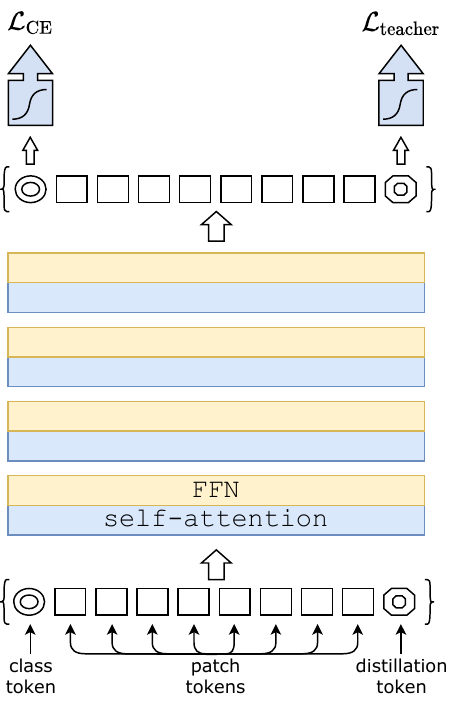
\includegraphics[width=0.5\linewidth]{img/DistillationToken}
        \caption[Distillation Token]{
            The figure from~\cite{touvron2021training}} shows how, similar to the [CLS] token, an additional distillation token is added to the transformer architecture.
        \label{fig:distillation-token}
    \end{figure}

    % flow: training the distillation token
    An already learned teacher network is used to train the distillation token.
    They use either the softmax output of the teacher network and try to minimize the Kullback-Leibler divergence between the outputs (soft distillation) or use the prediction of the teacher network as a label (hard distillation).
    Experiments have shown that hard distillation outperforms soft distillation.

    % flow: distillation token at inference
    To predict a label during inference, the average of the two softmax outputs is used.
    This gave better results than using either the class token or the distillation token alone.

    % flow: CNNs are better teachers
    They experimented with different teacher networks and found that the performed better with CNN teachers than with transformer teachers.
    One possible explanation for this is that they profit from the local restrictions of CNNs.

    % flow: distillation token add real value
    As a reference, a model with two [CLS] tokens was built.
    The first observation is that this didn't improve the performance of the model.
    More interesting, however, is the second observation that in this model the two randomly initialized [CLS] tokens converge to the same vectors, while in the distillation model the [CLS] token and the distillation token give different vectors after training.
    This shows that the distillation approach adds real value to the transformer.

% ==============================


    \section{Evaluation of the Transformers for image classification}\label{sec:evaluation-of-the-transformers-for-image-classification}
    % flow: experiments with mnist dataset
    In this chapter we demonstrate how the previously described transformers perform on image classification tasks.
    For this purpose, we use the well-known mnist dataset for comparison.
    It consists of images of 28x28 grayscale, handwritten digits and the task is to identify that digit.
    You can see an example image in figure~\ref{fig:mnist-example}.

    % flow: figure example mnist digit
    \begin{figure}[hbtp]
        \centering
        
\includegraphics[width=0.2\linewidth]{img/plots/patches/example}
        \caption[Mnist example]{Mnist example of a handwritten 2.}
        \label{fig:mnist-example}
    \end{figure}

    \subsection{Comparing the naive transformer with the Vision Transformer}\label{subsec:comparing-the-naive-transformer-with-the-vision-transformer}

    % flow: description first experiment
    First, we compare the naive transformer (see section~\ref{subsec:naive-transformer}) with the Vision Transformer (see section~\ref{subsubsec:vision-transformer}).
    As mentioned earlier, the naive transformer flattens the pixels of the image, embeds them and passes them into stacked transformer layers.
    The Vision Transformer, on the other hand, splits the image into patches, embeds them, and passes them into stacked transformer layers.
    Figure~\ref{fig:mnist-patches} illustrates how an mnist image is split into 4x4 patches.
    In figure~\ref{fig:flattened-mnist-patches} you can see the same patches in a flattened form.

    % flow: figure example mnist digit
    \begin{figure}[btp]
        \centering
        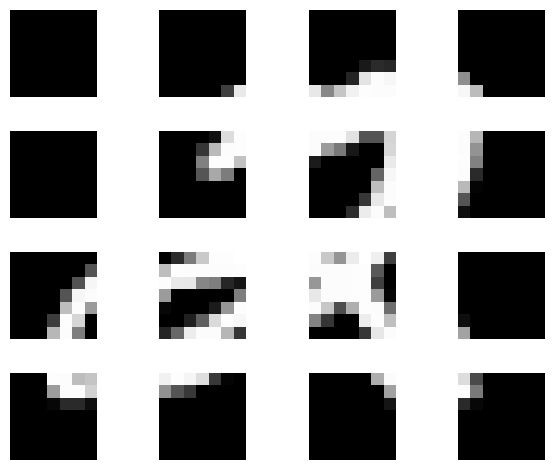
\includegraphics[width=0.2\linewidth]{img/plots/patches/example_tiles}
        \caption[Mnist example split into patches]{The image of the handwritten digit from above is split into patches.}
        \label{fig:mnist-patches}
    \end{figure}

    % flow: figure example mnist digit
    \begin{figure}[btp]
        \centering
        
\includegraphics[width=0.8\linewidth]{img/plots/patches/example_tiles_linear}
        \caption[Flattened patches of an mnist example]{The patches of the mnist example are flattened. This sequence is passed to the transformer layers.}
        \label{fig:flattened-mnist-patches}
    \end{figure}

    % flow: describe training
    To train the model, we used an Adam optimizer with a learning rate of 0.001 and exponential decay.
    All transformers are multi-head transformers which have 4 heads and an embeddings size of 4.
    The feed-forward layer has a hidden layer with 128 units.
    The models were trained for 5 epochs with a batch size of 8.
    Since the mnist images are of size 28x28, they cannot be split into 16x16 patches without remainders as proposed in the Vision Transformer paper~\cite{dosovitskiy2021image}.
    However, we can split then into 14x14 patches of size 2x2.
    As a further comparison, we added another Vision Transformer that splits the images into 4x4 patches of size 7x7.

    % flow: 7x7-Vision Transformer performed best
    In our experiments, we used a varying numbers of stacked transformer layers.
    In figure~\ref{fig:accuracies-naive-patch} you can see a plot with the number of transformer layers on the x-axis and the corresponding accuracy of each transformer on the y-axis.
    The 7x7 Vision Transformer performs best with some deviations.
    This is especially true considering that it gets the coarsest embedding of the images.

    % flow: more transformer layers only slight improvements
    After 15 transformer layers, no further performance improvement is apparent.

    % flow: figure accuracies of the naive transformer and the Vision Transformer
    \begin{figure}[btp]
        \centering
        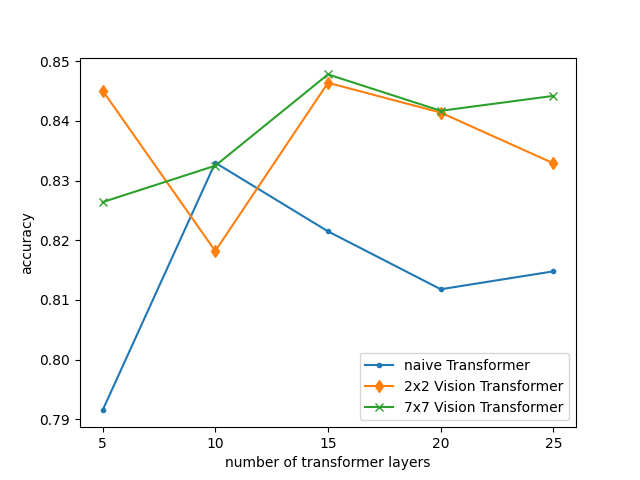
\includegraphics[width=0.8\linewidth]{img/plots/accuracies}
        \caption[Accuracies of the naive transformer and the Vision Transformer]{Accuracies of the naive transformer and the Vision Transformers plotted per number of transformer layer.}
        \label{fig:accuracies-naive-patch}
    \end{figure}

    % flow: niave more FLOPs
    In figure~\ref{fig:flops-naive-patch} you can see the number of floating point operations (FLOPs) needed for one image during inference.
    We have already explained in section~\ref{subsec:naive-transformer} that the computational complexity for the naive transformer is $\mathcal{O}(Ln^2)$, where $L$ is the number of transformer layers and $n$ is the number of pixels.
    The Vision Transformer has a complexity of $\mathcal{O}(Lp^2)$, where $p$ is the number of patches into which the image is divided.
    In our cases, we have $p = 196$ for the 2x2 Vision Transformer and $p = 16$ for the 7x7 Vision Transformer, since the images are split into 14x14 patches and 4x4 patches, respectively.
    Thus, we use only constant values for $p$ that are independent of $n$.
    Therefore, the complexity reduces to $\mathcal{O}(L)$.
    For all transformers, it increases linearly in the number of transformer layers, but the naive transformer consumes many more FLOPs than the Vision Transformers.

    % flow: figure flops naive transformer and Vision Transformer
    \begin{figure}[btp]
        \centering
        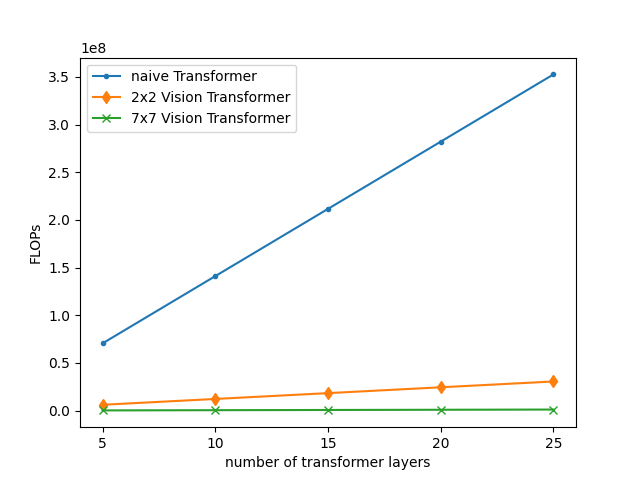
\includegraphics[width=0.8\linewidth]{img/plots/flops}
        \caption[Flops of the naive transformer and Vision Transformers]{Flops of the naive transformer and Vision Transformers per number of transformer layer}
        \label{fig:flops-naive-patch}
    \end{figure}

    % flow: paramter plot
    We also plotted the number of parameters needed for the transformers in figure~\ref{fig:num-params-naive-patch}.
    Again, the number of parameters increase linearly with the number of transformer layers, but there is only a constant difference between the naive transformer and the Vision Transformers.
    This is because the number of parameters of a transformer encoder cell is independent of the length of the input sequence, as we mentioned in section~\ref{subsubsec:multi-head-attention-section}.
    Only the positional embedding requires more parameters as the sequence length increases.

    % flow: figure parameter plot
    \begin{figure}[btp]
        \centering
        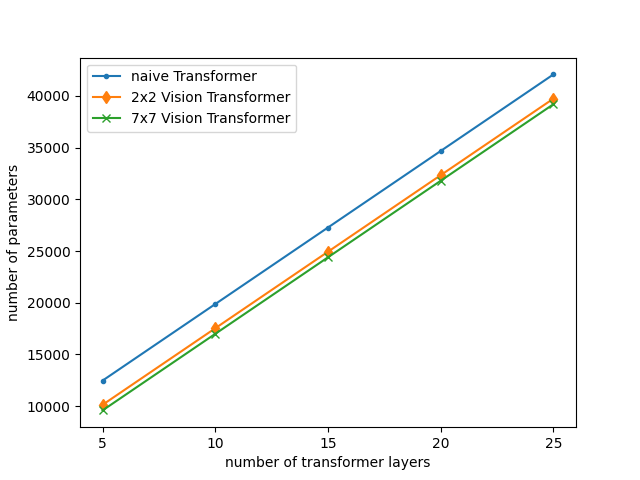
\includegraphics[width=0.8\linewidth]{img/plots/num_params}
        \caption[Number of parameters of the naive transformer and Vision Transformers]{Comparison of the number of parameter of the naive transformer and Vision Transformers.}
        \label{fig:num-params-naive-patch}
    \end{figure}

    \subsection{Comparing Vision Transformers to CNNs}\label{subsec:comparing-vision-transformers-to-cnns}
    % flow: compare vision transformers to CNNs
    In a second experiment, we compare vision transformers with the dominant approach in image processing, CNNs.

    % flow: transformer configuration
    We use multi-head attention transformers with 4 heads, an embedding dimension of 4 and a hidden layer with 128 units in the feed-forward section.
    We built transformers with 16, 32, 64, and 128 transformer layers.

    % flow: CNN configuration
    For the CNNs we used a hidden layer with 128 units in the decision head.
    We used a different number of convolutional layers and a different number of convolution kernels in each layer to create models with similar number of parameters as the transformers.
    In this way, we hope to make the comparisons as fair as possible.
    The different configuration of the convolutional layers are shown in table~\ref{tab:cnn-configurations}.
    All kernels of the convolutional layers were $3 \times 3$ kernels.


    \begin{table}[ht]
        \centering
        \begin{tabular}{ | c | c | c | }
            \hline
            number of parameters & number of transformer layers & number of convolutions \\
            \hline
            20k                  & 16                           & 4, 8, 16, 64           \\
            40k                  & 32                           & 8, 16, 32              \\
            90k                  & 64                           & 16, 32, 64             \\
            200k                 & 128                          & 16, 32, 64, 256        \\
            \hline
        \end{tabular}
        \caption[Configurations of the CNNs and Vision Transformers ]{
            Configurations of the CNNs and Vision Transformers.
            The leftmost column shows how the rough number of parameters of the models.
            The rightmost column shows the number of convolutions that are used in the different convolution layers.
            The first row means that the transformer in the 20k parameter category has 16 transformer layers.
            In the corresponding convolutional net, the first convolutional layer has 4 kernels, the second 8, the third 16 and the fourth 64.
        }\label{tab:cnn-configurations}
    \end{table}

    % flow: figure transformer CNNs comparision
    \begin{figure}[btp]
        \centering
        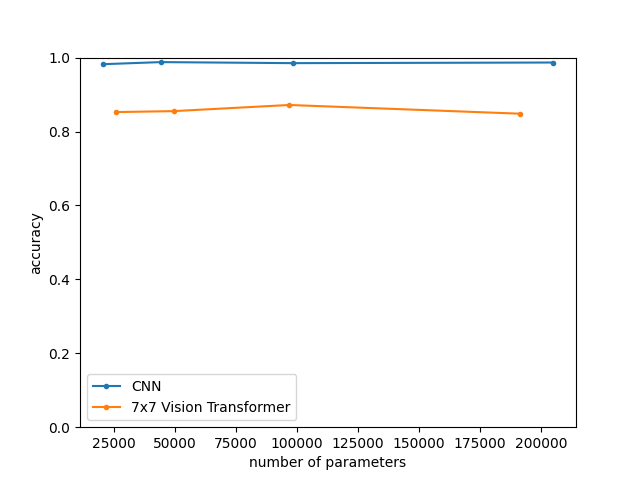
\includegraphics[width=0.8\linewidth]{img/plots/cnn-patch-comparison}
        \caption[Vision transformers compared to CNNs]{Accuracy of the Vision Transformer compared to a traditional CNN.
        The x-axis shows the number of parameters.
        The y-axis shows the accuracy of the models.
        }
        \label{fig:cnn-patch-comparison}
    \end{figure}

    % flow: CNNs outperform transformers in our example
    In figure~\ref{fig:cnn-patch-comparison} you can see the accuracy of the CNN and the Vision Transformer.
    The size of the model is not related to the accuracy in both cases.
    The CNN outperforms the Vision Transformer with an accuracy of 98\% compared to 86\%.

    % flow: dataset to easy
    One possible explanation is that the mnist dataset is a very simple dataset with few global dependencies to detect, so the transformer cannot show its advantages.

    % flow: need to learn inductive bias, more examples
    Another point is that transformers need a lot of examples to learn how to extract features from images, while this is given for CNNs through their internal structure.

    % flow: better performance with transfer learning
    Thus, CNNs perform better than transformers when both are trained from scratch.
    In the next section, we show how the performance of the transformers can be enhanced by transfer learning.

    \subsection{Transfer Learning with Transformers}\label{subsec:transfer-learning-with-transformers}
    % flow: intro transfer learning
    In transfer learning a pre-trained model is fine-tuned to a new dataset that has not yet been seen.
    Any pre-trained model, especially CNNs and transformers, can be used.

    % flow: pre-trained vision transformers
    We use pre-trained vision transformers on imagenet, the most commonly used dataset for transfer learning in image processing.
    In particular, we use the base and large configurations of the Visions Transformers with different number of patches.
    Since our input image are only of size 28x28, we scale them up to 32x32 pixels before training for all models.
    An overview of the configurations of the models is shown in table~\ref{tab:vit-configurations}.

    \begin{table}[ht]
        \centering
        \begin{tabular}{ | c | c | c | c | c | c |}
            \hline
            transformer & layers & embedding dim & mlp size & heads & number of patches \\
            \hline
            vit\_b16    & 12     & 768           & 3072     & 12    & 16x16             \\
            vit\_b32    & 12     & 768           & 3072     & 12    & 32x32             \\
            vit\_l16    & 14     & 1024          & 4096     & 16    & 16x16             \\
            vit\_l32    & 14     & 1024          & 4096     & 16    & 32x32             \\
            \hline
        \end{tabular}
        \caption[Configurations of the Vision Transformers used for Transfer Learning]{
            Configurations of the base (vit\_b) and large (vit\_l) vision transformers.
            The number at the end of the name refers to the number of patches into which the transformer splits the image.
            So the vitb\_32 transformer is a vision transformer in the base configuration which splits the image into 32x32 fix-sized patches.
            Content of the table taken from~\cite{dosovitskiy2021image}.
        }\label{tab:vit-configurations}
    \end{table}

    % flow: transfer learning experiment
    We add a new decision head to the pre-trained models and train the entire model with a learning rate of 0.0001 for two epochs with a batch size of 8.
    The results can be seen in figure~\ref{fig:transfer-learning-experiment}.
    All models performed very well, achieving all about 97\% accuracy.
    For our simple dataset, we did not see any significant differences between the different pre-trained transformers.
    However, as the datasets grow and become more complex, it might make sense to use the larger transformers if the computational cost is reasonable.

    % flow: figure transfer learning experiment
    \begin{figure}[btp]
        \centering
        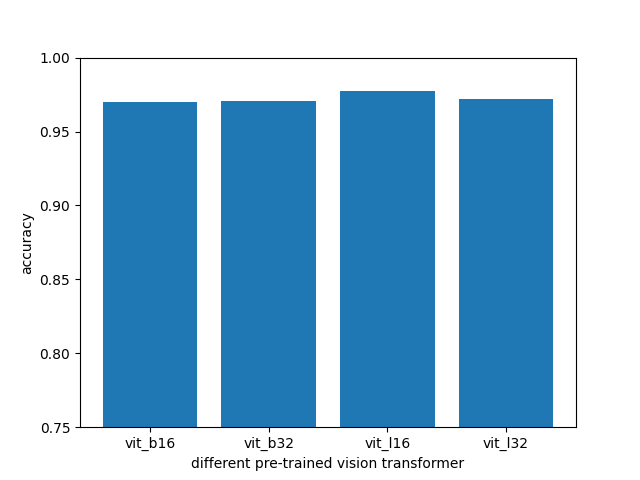
\includegraphics[width=0.8\linewidth]{img/plots/transfer_learning_transformer}
        \caption[Results of the transfer learning experiments]{Accuracies of the transformers trained with transfer learning.
        In table~\ref{tab:vit-configurations} you can see details about the pre-trained models.
        All models achieve a similar accuracy of about 97\%.
        }
        \label{fig:transfer-learning-experiment}
    \end{figure}

    % flow: compare to pre-trained CNN
    In the last section, we fine-tuned a CNN\@.
    It achieved an accuracy of just below 95\%.
    So transformers perform very well with transfer learning and can compete with CNNs.

    \subsection{Hybrid approaches of Transformers and CNNs}\label{subsec:hybrid-approaches-of-transformers-and-cnns}
    % flow: experiment for hybrid model
    Last but not least, we want to evaluate a hybrid approach combining CNNs and transformers.
    In section~\ref{subsec:hybrid-approaches} we described different approaches to such models.
    The common idea behind them is that CNNs better extract low-level features and transformers better add global context to them.
    All presented approaches modify the transformer architecture slightly.
    However, we would like to analyse this hypothesis independently.
    Therefore, we developed our own model which uses only a CNN and unmodified transformer layers.

    % flow: figure hybrid model
    \begin{figure}[btp]
        \centering
        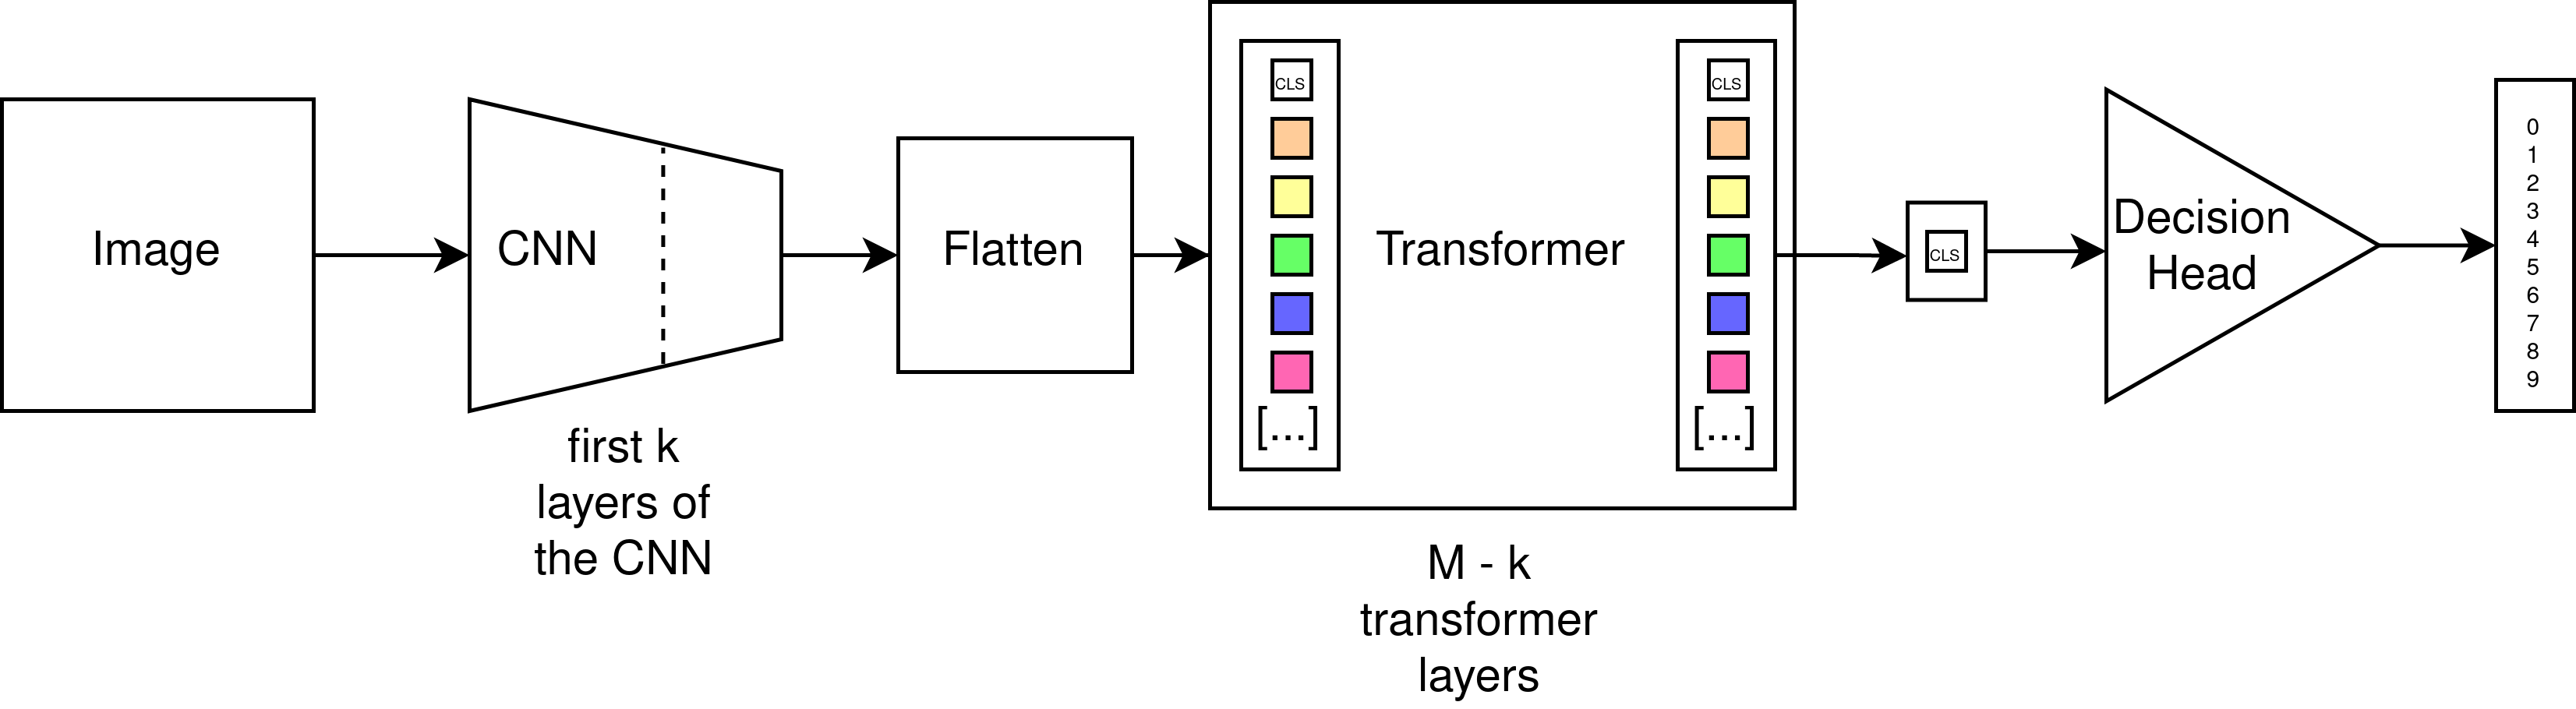
\includegraphics[width=1.0\linewidth]{img/HybridModelArchitecture}
        \caption[Architecture of the hybrid model]{Architecture of the hybrid model.
        The dashed line in the CNN part shows that only the first $k$ layers of this are taken.
            $M$ is the number of total layers of the CNN.
            The other $M - k$ layers of the CNN are replaced with transformer layers, for $k < M$.
            The first token of the transformer is the [CLS] token.
            Only the output of this is passed to the decision head which makes the final prediction.
        }
        \label{fig:architecture-hybrid-model}
    \end{figure}

    % flow: own model
    In figure~\ref{fig:architecture-hybrid-model} the architecture of our model is shown.
    The idea is to use a CNN to extract low-level features of the image and to further process them with a transformer.
    We use a pre-trained CNN for the feature extraction, but since we only want to extract low-level features, we do not use the whole network, but only the first $k$ layers of it.
    The extracted features are flattened and passed to a transformer encoder with a [CLS] token.
    The encoder consists of $M - k$ encoder cells, where $M$ is the total number of layers of the CNN\@.
    So, we preserve the total number of layers.
    The output of the [CLS] token is then used for classification.

    % flow: pretrained-model
    As a CNN, we choose the pre-trained VGG-16 model presented in~\cite{simonyan2015deep}.
    This model is a simple CNN consisting of stacked convolutional and pooling layers followed by a task-specific decision head.
    It consists of 16 weight layers, three of which are used for the classification head.
    Without these three layers, but with the five weightless pooling layers, there are 18 relevant layers left for transfer learning tasks.
    After each layer, the CNN is truncated and the truncated convolutional layers are replaced with transformer layers.
    Also, a new decision head is added to the model that gets the output of the convolutional layers.

    % flow: training details
    We experimented with different number of epochs, but found that only 2 epochs were sufficient for this transfer learning task.
    To train the model we used a batch size of 8 and a learning rate of 0.0001 and optimized all weights, not only the decision head.

    % flow: figure hybrid approaches
    \begin{figure}[btp]
        \centering
        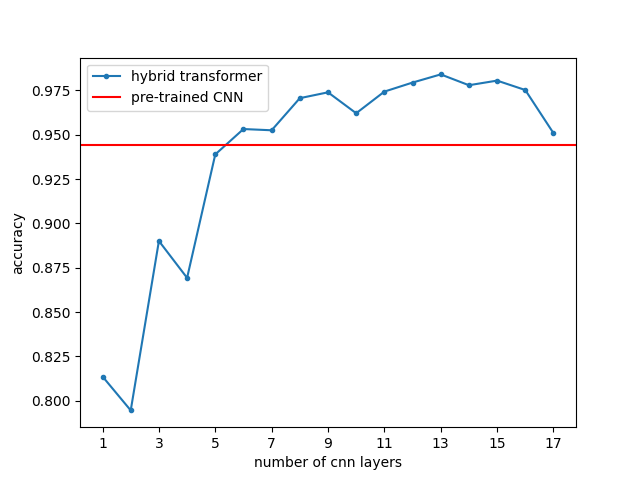
\includegraphics[width=0.8\linewidth]{img/plots/hybrid_transformer}
        \caption[Accuracy of hybrid approaches]{Accuracy of the hybrid models consisting of 18 layers in total.
        The x-axis shows the number of convolutional layers of the model.
        The rest of the 18 layers are transformer layers.
        The red line shows the accuracy of the pre-trained CNN with all 18 layers and no transformer layers.
        }
        \label{fig:hybrid-accuracy}
    \end{figure}

    % flow: evaluaton hybrid model
    In figure~\ref{fig:hybrid-accuracy} you see the accuracy of the trained models.
    The red line shows the accuracy of the pre-trained CNN fine-tuned to the mnist dataset.
    Here, we only added a new decision head and no transformer layers.
    The important observation is that on the left side, where we use only a few convolution layers followed by many transformer layers, the performance is worse than the pre-trained CNN\@.
    Only in the middle where 6 up to 17 convolution layers are followed by corresponding 12 to 1 transformer layers, the hybrid approach outperforms the pre-trained CNN\@.
    The right end of the curve approaches the red line as the models become more similar.

    % flow: interpretation of the plot
    This proves that convolutions are good at extracting low-level features from the image, but lack at putting them into global context.
    But this is exactly the strength of the transformer.
    So using the hybrid approach with the right number of convolutional layers performs better than each model on its own.

% ==============================


    \section{Visualizing attention}\label{sec:visualizing-attention}
    % flow: intro visualizing attention
    Another exiting aspect of transformers is that one can visualize attention and thus create a mechanism to explain the decisions of the net.
    This is a step towards Explainable AI, which gets more and more important and is a major area of current research.
    Visualization techniques also exist for CNNs, but they only focus on which pattern the kernel provides the largest activation for.
    However, this can be done only once for the net and not individually for each image.

    % flow: different approaches
    We present two approaches for attention visualization, called Attention Rollout and Attention Flow, both from~\cite{abnar2020quantifying}.
    However, there is also a second category of visualization techniques presented in~\cite{chefer2021transformer} which computes local relevancy scores for each token and propagates them heuristically through the attention graph.
    They perform slightly better, but build on Attention Rollout and Attention Flow.

    % flow: difference to Attention Rollout
    Empirical comparison of Attention Rollout and Attention Flow has shown that Attention Flow better distinguishes between relevant and irrelevant tokens for the decision, but Attention Rollout provides the better discrimination between them.
    Both can be computed in polynomial time, but Attention Rollout is a bit faster with $\mathcal{O}(Ln^2)$ time compared to $\mathcal{O}(L^{2}n^4)$ time for Attention Flow, where $L$ is the number of transformer layers and $n$ is the number of tokens.

    \subsection{Attention Rollout}\label{subsec:attention-rollout}
    % flow: raw attention weight matrix
    In section~\ref{subsubsec:multi-head-attention-section} we described how the attention is calculated inside the transformer.
    Let us repeat the main equation, equation~\ref{eq:scaled-dot-mat}, of this calculation:
    \begin{equation}
        \text{ScaledDotProductAttention}(X) = \text{softmax}(\frac{QK^T}{\sqrt {d_k}})V \label{eq:scaled-dot-mat-repeat}
    \end{equation}

    We introduce the raw attention matrix $\hat{W}$ as the output of the softmax calculation:
    \begin{equation}
        \hat{W} = \text{softmax}(\frac{QK^T}{\sqrt {d_k}})
    \end{equation}

    Thus, we can write equation~\ref{eq:scaled-dot-mat-repeat} as:
    \begin{equation}
        \text{ScaledDotProductAttention}(X) = \text{softmax}(\frac{QK^T}{\sqrt {d_k}})V = \hat{W}V \label{eq:scaled-dot-mat-w}
    \end{equation}

    % flow: goal of Attention Rollout
    The goal of Attention Rollout (see~\cite{abnar2020quantifying}) is to combine the matrices $\tilde{W}$ of the different transformer layers and of the different attention heads inside a layer into a single matrix.
    The first row of this combined matrix corresponds to the attention weights of the [CLS] token and these values are visualized.
    For this purpose they are taken and arranged as in the original image.
    Each value is a weight for a patch into which the image was split.
    For each pixel of the image, the weight of its patch is used.
    The values are interpolated to obtain smooth transitions between them.
    These are the final values for the visualization.

    % flow: images of attentin visualizations
    \begin{figure}[btp]
        \centering
        \begin{subfigure}[t]{0.3\textwidth}
            \centering
            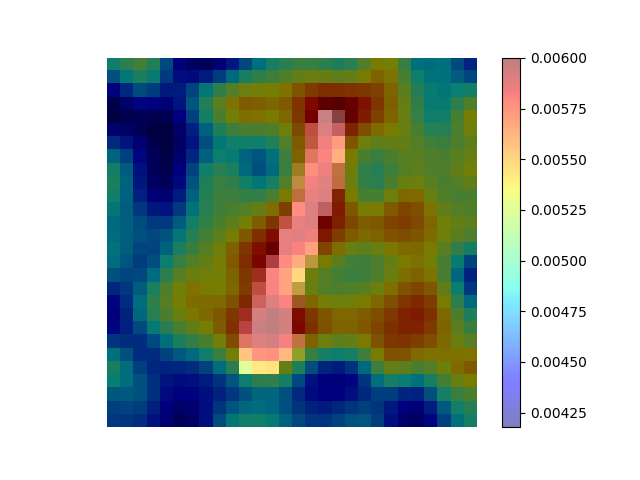
\includegraphics[width=\textwidth]{img/plots/attention_visualization_good_1}
        \end{subfigure}
        \hfill
        \begin{subfigure}[t]{0.3\textwidth}
            \centering
            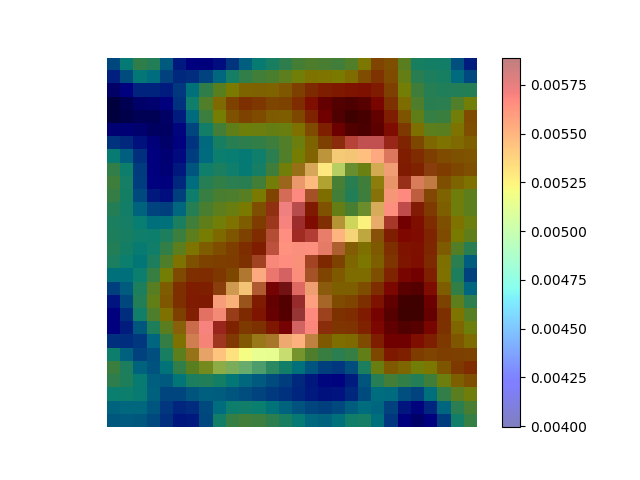
\includegraphics[width=\textwidth]{img/plots/attention_visualization_middle_1}
        \end{subfigure}
        \hfill
        \begin{subfigure}[t]{0.3\textwidth}
            \centering
            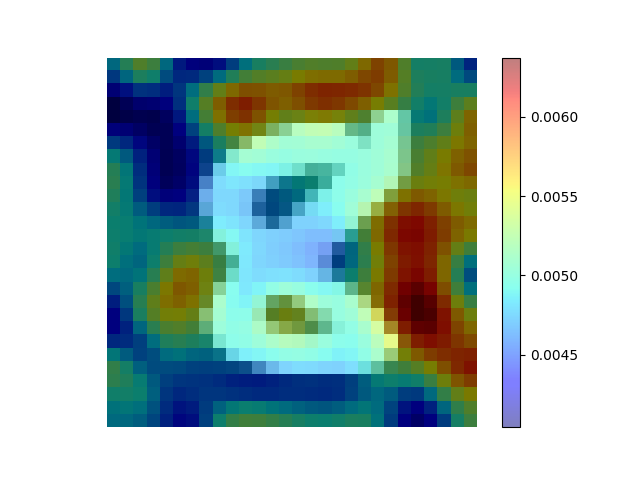
\includegraphics[width=\textwidth]{img/plots/attention_visualization_bad_1}
        \end{subfigure}

        \begin{subfigure}[t]{0.3\textwidth}
            \centering
            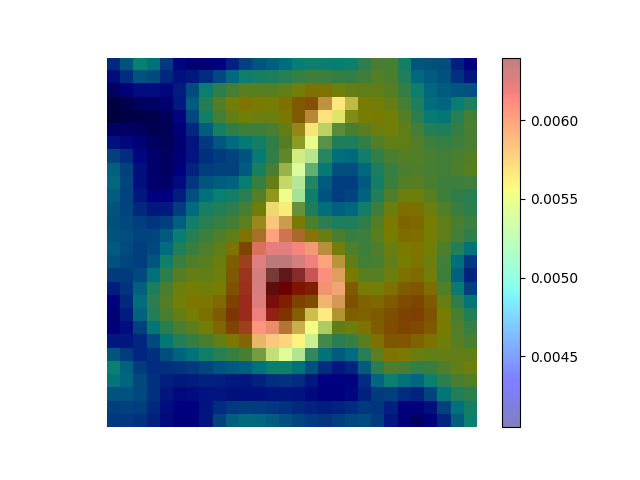
\includegraphics[width=\textwidth]{img/plots/attention_visualization_good_2}
            \caption{clear}
        \end{subfigure}
        \hfill
        \begin{subfigure}[t]{0.3\textwidth}
            \centering
            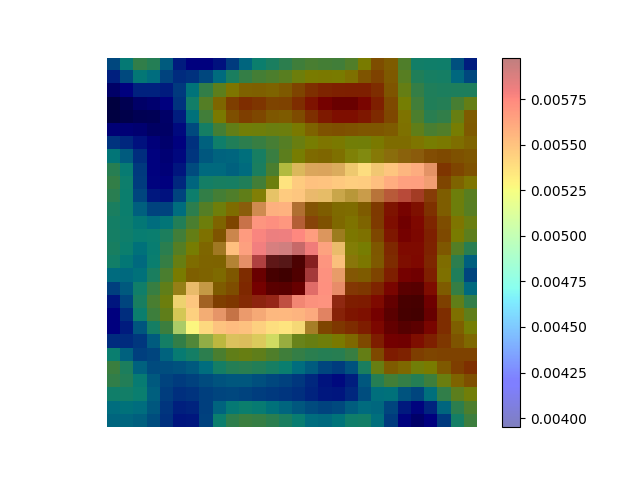
\includegraphics[width=\textwidth]{img/plots/attention_visualization_middle_2}
            \caption{intermediate}
        \end{subfigure}
        \hfill
        \begin{subfigure}[t]{0.3\textwidth}
            \centering
            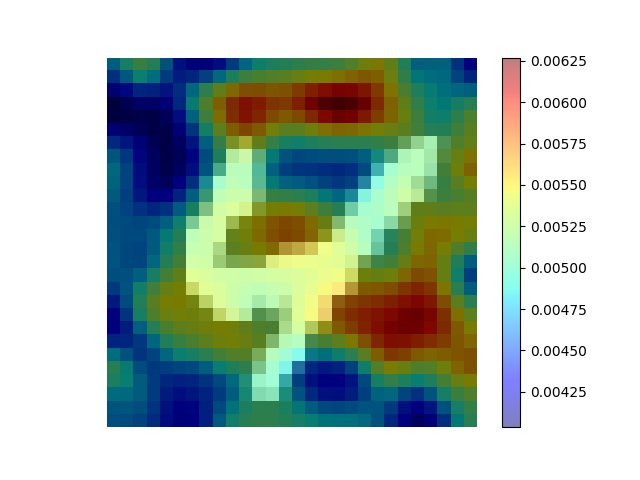
\includegraphics[width=\textwidth]{img/plots/attention_visualization_bad_2}
            \caption{unclear}
        \end{subfigure}
        \caption[Examples of clear and unclear attention visualizations for mnist digits]{Examples of clear, intermediate and unclear attention attention visualizations for mnist digits. The red regions correspond to regions of high attention, the blue to regions of low attention.}
        \label{fig:attention-visualization}
    \end{figure}

    % flow: attention visualiztion
    In figure~\ref{fig:attention-visualization} examples of attention visualizations are given for correctly classified mnist digits.
    The red regions correspond to regions of high attention, the blue to regions of low attention.
    There are two clear examples in the left column.
    Here you can see that the red regions form the shape of the digits.
    There are areas of lower attention, marking the edges of it.
    The digits in the center are also roughly covered by red regions but there are also red regions outside the digits.
    With some creativity, one can interpret the visualizations, but the results are not as clear as on the left side.
    For example, in the case of the eight on the top, one can argue that the transformer has detected the top of the digit and that it is tilted.
    It looks in both directions, to the left and to the right, where the digit continues.
    This adds kind of temporary relations into the visualization that cannot be derived from it.
    The right column shows two examples where the shapes of the digit and the regions of high attention do not match.
    Here it is very difficult to make sense of them.

    % flow: static noise
    If one looks carefully at the images, one can see similar patterns in all visualizations.
    For example, there is always a region of low attention in the upper left corner.
    And there is also an elongated region of low attention in the bottom of all images.
    This can be interpreted as the search pattern that the transformer learned for the mnist digits.

    % flow: cherry-picked examples
    The examples are cherry-picked, but most fall into the left or middle categories.
    Now, we describe how to calculate the values for the visualizations.

    % flow: combine heads
    The first step to obtain the final combination matrix is to combine the raw attention matrices $\tilde{W}$ of the heads.
    One approach is to use the average of the matrices of the heads.
    Other aggregation functions, like taking the minimum or maximum, are also valid choices.
    It is also possible to consider each head individually.
    Regardless of how the matrices of the heads are combined, we normalize the resulting matrix and call it the attention weight matrix $W$.
    For each $l = 1, \dots, L$ where $L$ is the number of transformer layers, $W_l$ is the attention weight matrix of the transformer layer $l$.

    % flow: combination of the layers
    In each transformer layer $l$, its value matrix $V_l$ is multiplied by the attention weight matrix $W_l$ within the scaled dot-product attention.
    Via the residual connection, the result of this is added to the input sequence.
    If we ignore the feed-forward sections after the multi-head attention section and do not distinguish between the input sequence and the value matrix, that is derived from it, we arrive at the following equation:

    \begin{equation}
        V_{l+1} = W_l V_l + V_l = (W_l + \mathds{1})V_l
    \end{equation}

    % flow: simplifications may not lead to exact results
    The simplifications we have made to retrieve this equation are not negligible and should always be considered when looking at Attention Rollout visualizations.

    % flow: attention weight matrix
    We define now the raw attention matrix $\tilde{A}_l$ as the normalization of $W_l + \mathds{1}$ such that the rows sum up to $1$.
    For all $l$ this is already given for $W_l$ by definition.
    So by adding $\mathds{1}$, each column sums up to $2$, and therefore we have to take half of each matrix, giving the following equation for $\tilde{A}_l$:

    \begin{equation}
        \tilde{A}_l = \frac{1}{2} W_l + \frac{1}{2} \mathds{1}
    \end{equation}

    Now we can combine the different raw attention matrices into the attention matrix by 'rolling them out'.
    The attention matrix $A_l$ for each layer is calculated by multiplying the raw attention matrix $\tilde{A}_l$ by the attention matrix of the previous layer $A_{l-1}$ or, in the case of the first layer, by the raw attention matrix $\tilde{A}_l$ itself, i.e.

    \begin{equation}
        A_l = \begin{cases}
                  \tilde{A}_l * A_{l-1}& \text{if $l > 1$}\\
                  \tilde{A}_l& \text{if $l = 1$}\\
        \end{cases}\label{eq:_3}
    \end{equation}

    $A_L$, the attention matrix of the last layer, is the final combination of all raw attention matrices.
    Its first row is extracted and visualized.

    \subsection{Attention Flow}\label{subsec:attention-flow}
    % flow: description flow network
    Another approach for attention visualization is Attention Flow (see also~\cite{abnar2020quantifying}).
    Here, transformer architecture is treated as a flow network.
    Such a network consists of an acyclic directed graph together with a capacity function that assigns a positive real value to each edge of the graph.
    There are two special nodes the source $s$ and the target $t$.
    To imagine such a network you can think of a network of water pipes.
    The capacity function models the size of the pipes and the source is a water source from which it flows through the pipes to the target.

    % flow: flow
    In such a network, finding a maximum flow is an interesting problem.
    A flow is a function that assigns a real value to each edge and satisfies the capacity and flow constraint.
    The capacity constraints states that the flow assigned to an edge must be positive and can not exceed the limit defined by the capacity function.
    The flow constraint models that the same amount entering a node must leave it.
    A maximum flow is a flow at which the capacity limit is reached on at least on edge on each path from $s$ to $t$.

    % flow: copute maximum flow
    An algorithm for computing a maximum flow can be found in~\cite{goldberg1988anew}, where an overview of previously known algorithms is also given.

    % flow: figure attention graphs
    \begin{figure}[btp]
        \centering
        \begin{subfigure}[t]{0.4\textwidth}
            \centering
            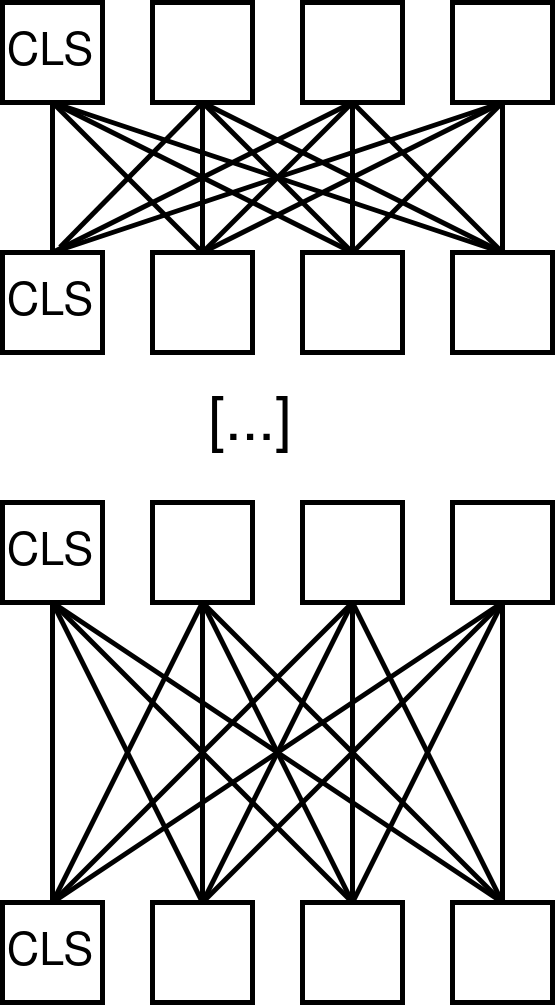
\includegraphics[width=0.5\textwidth]{img/AttentionGraph}
            \caption{Attention connections}
        \end{subfigure}
        \hfill
        \begin{subfigure}[t]{0.4\textwidth}
            \centering
            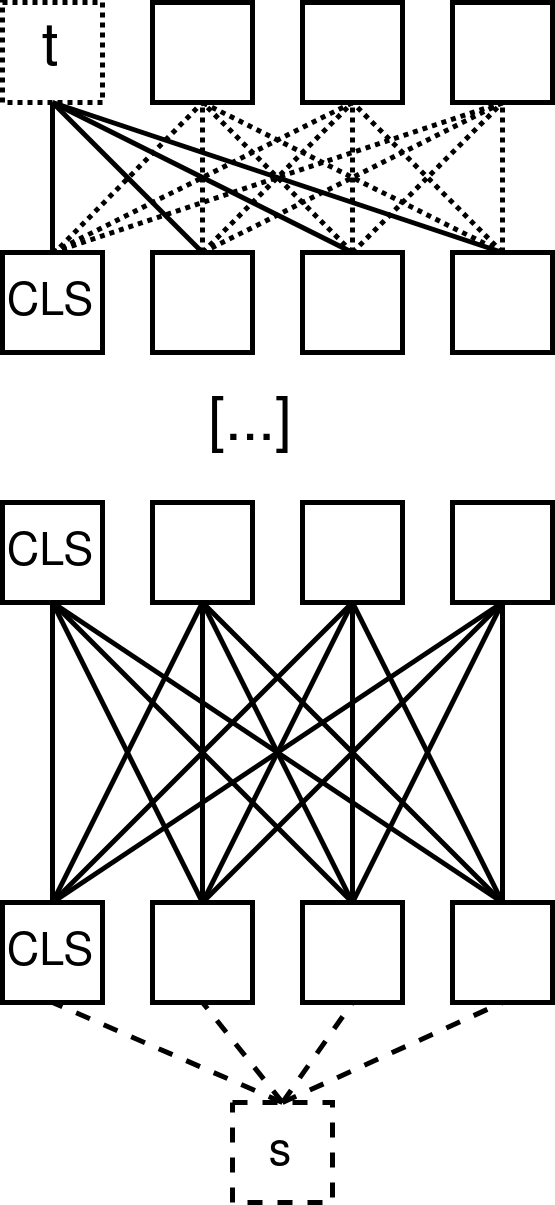
\includegraphics[width=0.5\textwidth]{img/AttentionFlowGraph}
            \caption{Attention flow network}
        \end{subfigure}
        \caption[Attention connections and Attention Flow network]{
            Attention connections and Attention flow network.
            On the left the attention connections between the tokens of the different layers are shown.
            The right shows the corresponding flow network.
            The dashed lines at the bottom show how a source token is added.
            The dotted lines at the top show the $t$ token and that only the connections to this are considered.
        }
        \label{fig:attention-flow-network}
    \end{figure}

    % flow: transformer as flow network
    The values of the transformer blocks are now seen as the nodes of the flow network.
    And the raw attention weight matrices $\tilde{A}_l$ between them represents the capacity function.
    On the left of figure~\ref{fig:attention-flow-network} the connections between the tokens are visualized.
    The right side of this figure shows how this is converted into a flow network.
    The changes are drawn in dashed or dotted lines.
    A source token is added before the first transformer layer.
    The target token is the [CLS] token of the last layer.
    Only the connections to this token are considered.
    A maximum flow for this graph is calculated and the minimum on each path from an input token to the [CLS] token is determined.
    These values are summed up for each input token and form the final values.

% ==============================


    \section{Transformers in other image processing applications}\label{sec:transformers-in-other-image-processing-applications}
    % flow: intro chapter
    So far, we have seen that transformers can be successfully used for image classification.
    In this chapter, we show some examples of how transformers are also used in other image processing applications.
    We start with object detection and segmentation tasks, which we explain in more detail.
    After that, we briefly discuss other areas.

    \subsection{Object Detection \& Segmentation Tasks}\label{subsec:object-detection}
    % flow: intro different tasks
    First, we describe the different tasks of segmentation and object detection tasks.

    \subsubsection{Explanation of object detection and the segmentation problem}
    % flow: differentiate problems
    In figure~\ref{fig:segmentation-tasks} you can see an example image and the corresponding output for the different tasks.
    The input image in the upper left can be any image.
    In the other images the outputs for semantic segmentation, instance segmentation and panoptic segmentation are visualized.

    % flow: figure segmentation problems
    \begin{figure}[hbtp]
        \centering
        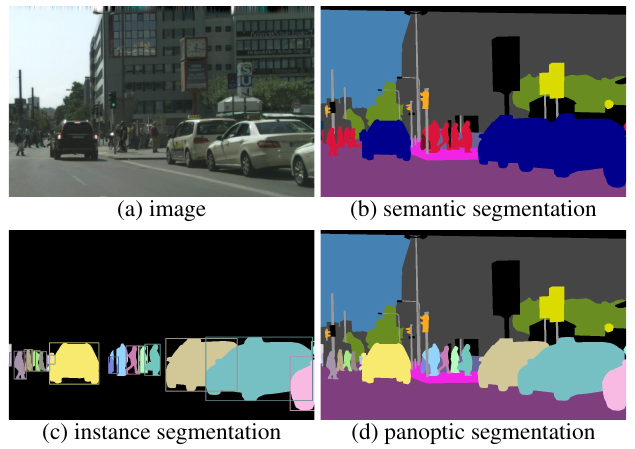
\includegraphics[width=0.5\linewidth]{img/SegmentationTasks}
        \caption[Different Segmentation Tasks]{Overview of the different segmentation tasks.
        The upper left shows an example input images and the other images are the outputs for the specific tasks.
        Figure is from~\cite{kirillov2019panoptic}}
        \label{fig:segmentation-tasks}
    \end{figure}

    % flow: semantic segmentation
    In semantic segmentation, each pixel is assigned one of a fixed set of classes.
    It is important to note that two instances of the same class have the same label and therefore cannot be distinguished.

    % flow: object detection
    The goal of object detection is to identify different objects with bounding boxes and to classify them.
    In this case, different objects of the same class would get different bounding boxes and thus can be told apart.
    Now, not all pixels in the image are categorized because, it is pointless to try draw bounding boxes around things in the background.
    An example of these bounding boxes are shown in (c) of the figure.

    % flow: instance segmentation
    Instance segmentation is like object detection, but instead of identifying the objects with bounding boxes the task is to determine the exact pixels of the object.
    Again, different instance of the same class would receive different labels, while the unobtrusive objects remain unclassified.

    % flow: panoptic segementation
    Panoptic segmentation is the combination of the two segmentation tasks.
    The goal is to classify each pixel while distinguishing multiple instances of the same class.
    Formally, this is achieved by assigning to each pixel a label $(c, i)$ consisting of the predicted class $c$ and an object identifier $i$.

    \subsubsection{Object Detection with Transformers}
    % flow: figure architecture DETR
    \begin{figure}[btp]
        \centering
        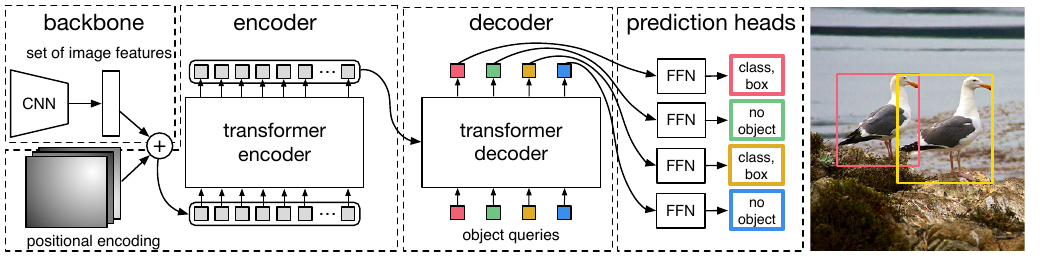
\includegraphics[width=1.0\linewidth]{img/DetrArchitecture}
        \caption[DETR Architecture]{DETR Architecture.
        A CNN computes features of the input image.
        These are passed to a transformer encoder.
        A transformer decoder receives object queries and outputs all detected objects at once.
        The outputs of the decoder are passed to a feed forward network to compute the bounding boxes and classify the object.
        Since the transformer outputs always a fixed number of tokens, there is a special no-object class that states that this output should not be considered.
        Figure is from~\cite{carion2020endtoend}}
        \label{fig:detr-architecture}
    \end{figure}

    % flow: DETR architecture
    DETR (DEtection TRansformer)~\cite{carion2020endtoend} is one approach for detecting objects with transformers.
    Its architecture is shown in figure~\ref{fig:detr-architecture}.
    It consists of an CNN that extracts features from the image.
    These are passed to an transformer architecture, that is almost identical to the original NLP transformer architecture.
    The transformer encoder is a normal encoder cell, before which a positional encoding is added to the extracted features.
    The transformer decoder is also quite similar to the original, except that it predicts the bounding boxes all at once at training and inference, instead of sequentially generating the next token.
    The input to the decoder are so-called object queries which are different learned vectors to generate different output predictions.
    Each output token of the decoder is interpreted as one object.
    The final class prediction and bounding box calculation is done by an additional feed forward network.
    Since the transformer architecture always predicts a fixed number of objects, there is a special 'no object' class that indicated that there is no object and that the loss of the bounding box should not be taken into consideration.

    % flow: interpretation of model
    Here, similarities to the previously described models for image classification and NLP applications can be seen.
    First, a CNN is used to extract features from the image.
    Second, a transformer encoder cells add global context to them.
    Since object detection involves generating bounding boxes, transformer decoder cells are used for this purpose, as in the original transformer model presented in section~\ref{subsec:transformer-architecture}.

    % flow: DETR loss
    To train the model, a loss value is used that compares the predicted bounding boxes with the ground truth.
    Both the predicted class and the bounding boxes are token into account.

    % flow: DETR advantages
    DETR is characterized by the simplicity of its architecture which is almost identical to that of the original transformer.
    It also does not require non-maximum suppression like many other approaches such as~\cite{dumitru2014scalable},~\cite{lin2018focal} or~\cite{wei2016single}.
    Non-maximum suppression is a post-processing step that removes similar low confidence bounding boxes and keeps only the one with the highest confidence.
    This is to prevent one object from being detected multiple times with different bounding boxes.

    % flow: DETR visualization
    Again, by visualizing the attention of the transformer one gets insights in the decision-making of the model.
    In figure~\ref{fig:detr-visualization} this is done for an example image with two elephants.
    The regions with high attention scores are draws in color and one can clearly see that these correspond to the parts of the elephant that determine the bounding box.

    % flow: DETR visualization
    \begin{figure}[btp]
        \centering
        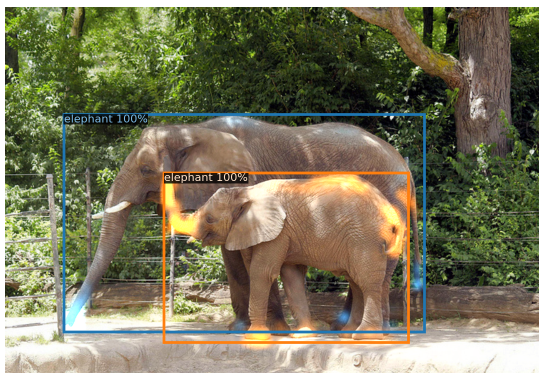
\includegraphics[width=0.7\linewidth]{img/DetrVisualization}
        \caption[DETR Visualization]{Visualization of attention maps of DETR\@.
        Colored regions correspond to regions with high attention.
        The transformer assign high attention scores to parts of the object on the edges.
        Image is taken from~\cite{carion2020endtoend}}
        \label{fig:detr-visualization}
    \end{figure}

    \subsection{Image Generation}\label{subsec:image-generation}
    % flow: intro image generation
    In section~\ref{subsubsec:image-transformer} we have already explained how~\cite{parmar2018image} restricts the attention within the transformer to local 1D or 2D areas.
    This model was originally developed for image generation.
    However, the attention mechanism can also be used for classification.
    One task of image generation is to generate images for a particular class from scratch, but there are also other tasks, e.g.\ completing a partial image or recovering high-resolution images from low-resolution representations.

    % flow: iGPT
    Another approach to image generation is image GPT (iGPT)~\cite{chen2020generative}, which uses the same architecture as the GPT-2 model~\cite{radford2019language} that was designed for NLP\@.
    The GPT-2 model consists only of stacked transformer decoder cells and is trained to complete a given input sequence.
    This can also be used for the image domain.
    Here, the images are flattened into sequences of pixels and the model is trained to predict the next ones.
    Due to the high computational complexity of this approach, this was only demonstrated for images with low resolutions.
    The intermediate representation of the images were examined and classifications based on them were found to be competitive with the top CNNs.

    \subsection{Text to image generation}\label{subsec:text-to-image-generation}
    % flow: text to image generation
    In the previous section, image generation was done by completing images.
    A similar task is to create image from text.
    In~\cite{ramesh2021zeroshot} this is achieved in two stages.
    The first stage uses an auto-encoder to compress the images.
    The second stage consists of an auto-regressive transformer that uses the concatenation of the encoded text and the compressed image tokens as input.
    The model can generate image from scratch or complete given images parts.

    \subsection{Image Captioning}\label{subsec:image-captioning}
    % flow: intro image captioning
    Image Captioning is exactly the other way round.
    Here, descriptions for given images are generated.
    Figure~\ref{fig:image-captioning-architecture} shows the architecture of a model presented in~\cite{he2021image} for image captioning with transformers.
    At first, a Faster-RCNN is used to detect important regions in the image.
    These regions are then fed into a spatial graph transformer.
    This is a modified transformer that relates and transforms the regions.
    Finally, a transformer decoder in combination with an LSTM cell is used to generate the output.

    % flow: figure image captioning architecture
    \begin{figure}[btp]
        \centering
        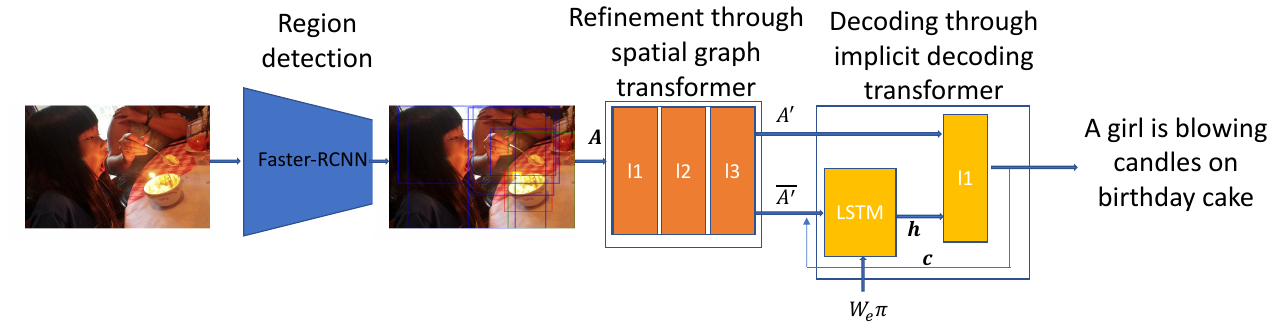
\includegraphics[width=1.0\linewidth]{img/ImageCaptioningArchitecture}
        \caption[Image Captioning Architecture]{Image Captioning Architecture.
        A Faster-RCNN is used to detect important regions.
        A spatial graph transformer is used to further process these regions.
        An LSTM cell and a transformer a used to generate the caption for the image.
        Figure is taken from~\cite{he2021image}}
        \label{fig:image-captioning-architecture}
    \end{figure}

% ==============================


    \section{Should Transformers replace convolutions?}\label{sec:should-transformers-replace-convolutions?}
    % flow: intro should transformers replace convolutions
    In our experiments, we have seen the promising results that transformers can compete with CNNs.
    This raises the question of which will prevail in the future.
    To answer this we will combine our findings with some literature on this subject.

    \subsection{Transfer Learning}\label{subsubsec:transfer-learning}
    % flow: out experiments
    In the experiment presented in section~\ref{subsec:comparing-vision-transformers-to-cnns}, we trained transformers and CNNs from scratch.
    Here, CNNs performed better than transformers.
    In section~\ref{subsec:transfer-learning-with-transformers} we used pre-trained transformers and fine-tuned them to our dataset.
    Thereby, the transformers achieved better results than the transfer learning with CNNs.

    % flow: transfer learning with CNNs and transformers
    In~\cite{zhou2021convnets} a more detailed study about the transfer learning capabilities of transformers and CNNs was conducted.
    Models were pre-trained on ImageNet and compared with models with similar top-1 on several downstream tasks.
    The overall result was, that the pre-trained and fine-tuned transformers lead to better results.
    In particular, when the domain is very different from ImageNet, transformers outperformed CNNs.

    % flow: transformer pre-training in medical domain
    In~\cite{matsoukas2021isit} the same topic was discussed in the field of medical images.
    The above results that pre-trained transformers on Imagenet are as good as conventional CNNs or even slightly better in transfer learning were confirmed.
    However, when training from scratch, CNNs are still the better solution because transformers require more data and training time.

    \subsection{Additional benefit of attention visualization}\label{subsec:additional-benefit-of-attention-visualization}
    % flow: intro benefit of attentin visualization
    In chapter~\ref{sec:visualizing-attention} we showed how to visualize the attention for our mnist example.
    This gave us insights into the network and helped us to understand its decisions.
    This shows its full value, when it comes to real-world domains, such as medical images.
    Doctors can improve their analysis by using a classification transformer and validating their results by comprehending the network's decisions.
    In addition, the visualizations increase the trust in the network, as it is no longer just a black box.
    In~\cite{matsoukas2021isit} the interpretability of CNNs and transformers is compared for medical images.

    % flow: figure medical visualization
    \begin{figure}[btp]
        \centering
        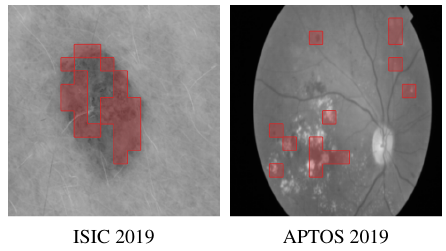
\includegraphics[width=0.8\linewidth]{img/MedicalVisualization}
        \caption[Attention Visualization on medical images]{Attention Visualization of medical images.
        The left image is an example of the ISIC 2019 dataset which is about skin cancer detection.
        The right image shows an example of the APTOS 2019 dataset which is about detection diabetic retinopathy to prevent blindness.
        Images are taken from~\cite{matsoukas2021isit}}.
        \label{fig:medical-visualization}
    \end{figure}

    % flow: ISIC image
    In figure~\ref{fig:medical-visualization} you can see two examples of images of medical examples and the corresponding visualized attention.
    On the left is an example of the ISIC 2019 dataset\footnote{\href{https://challenge2019.isic-archive.com/}{https://challenge2019.isic-archive.com/}}, a dataset about skin cancer detection.
    Using a transformer trained on it and insight into its decisions could greatly help physicians detect skin cancer more accurately.

    % flow: APTOS image
    APTOS 2019\footnote{\href{ihttps://www.kaggle.com/c/aptos2019-blindness-detection/overview/aptos-2019}{https://www.kaggle.com/c/aptos2019-blindness-detection/overview/aptos-2019}} is a dataset for detecting diabetic retiopathy in the early to stage to prevent blindness.
    On the right site of the figure, you can see an example of this dataset which visualized attention.
    Currently, the vast amounts of images are analyzed by highly specialized doctors.
    In the future, this could change and an artificial model could make a preselection.
    Images for which the model is not confident enough will be further evaluated by physicians.
    However, with the help of a transformer model and its visualization, this process could be accelerated and the resources for this task reduced.
    All this lowers preventive healthcare costs and reduces the number of diabetic retinopathy causing blindness.

    \subsection{Convolutions in early layers}\label{subsec:convolutions-in-early-layers}
    % flow: hybrid solution perform best
    In~\cite{wu2021visual} the use of convolutions in early layers of transformers is discussed.
    It is argued that convolutions are designed to detect low-level features like edges or corners, while transformers are very inefficient at such detections and require more data to be trained for them.
    Therefore, CNNs should be used in the early layers while in later stages it is advantageous to use transformers.
    There are several reasons for this, but one of them is that convolutions in later stages are specialized for high-level features that are sparse in varying domains.

    % flow: figure attention distance
    \begin{figure}[btp]
        \centering
        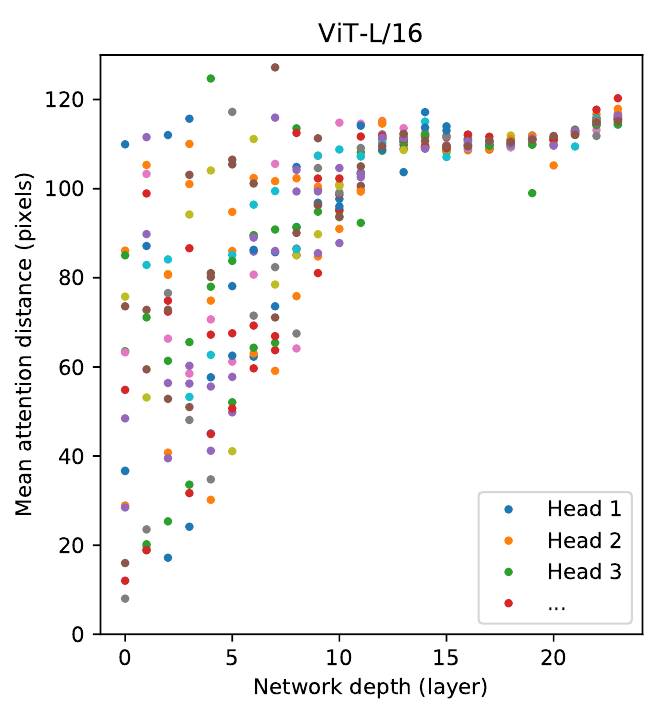
\includegraphics[width=0.6\linewidth]{img/AttentionDistance}
        \caption[Attention distance]{Plot of the mean attention distances of the different attention heads at different network depths.
        Attention heads in the early layers show low and high mean attention distances whereas in the later layers all attention heads have high attention distances.
        Figure is taken from~\cite{dosovitskiy2021image}}
        \label{fig:attention-distance}
    \end{figure}

    % flow: transformers in early layers
    In figure~\ref{fig:attention-distance} the mean attention distance is plotted on different network layers of a vision transformer.
    As you can see, in the early layers most of the heads attend only to local pixels.
    Such attention heads could be easily replaced by convolutions.
    In the later layers, all attentions heads have a large attention distance.
    Here, the full potential of the transformer architecture is exploited.
    However, in the early layers there are also some attention heads attending to distant pixels.

    % flow: convolutions lead to more stability
    In~\cite{xiao2021early} the splitting of the image into patches of the Vision Transformer is interpreted as a large, strided convolution.
    There it is showed, that the model converges faster when this is replaced with smaller convolutions with a loser stride, and that is has then a higher weight decay stability.

    % flow: our experiment
    All this motivated our experiment of section~\ref{subsec:hybrid-approaches-of-transformers-and-cnns}.
    There we replaced the convolution layers of a pre-trained CNN with transformer layers.
    We were able prove the statement that the network benefits from convolutions in early layers.
    Furthermore, we extended this to the fact that the performance decreases when replacing too much transformer layers with convolutions.

    % flow: summary hybrid models
    In summary, it makes sense to replace the early layers of a transformer with convolutions when only a small amount of data is available and a faster training is important.
    However, this has the disadvantage that visualization of attention is no longer possible.
    The convolutions in the first layers limit the model to detecting local dependencies in these layers, which could be detrimental to more complex examples but was not the case in our experiments.

    \subsection{Transformers are more intuitive}\label{subsec:transformers-are-more-intuitive}
    % flow: transformers are more human-like
    In~\cite{tuli2021are} a comparison of CNNs and transformers is made to see which behaves more human-like.
    The results were that CNNs classify more by texture and that transformers and humans classify more by shape.
    They also compared which images the models made errors on, and concluded that the errors of transformers and humans were more consistent than those of CNNs and humans.
    This makes transformers more understandable and is another step towards Explainable AI\@.

    % flow: not all pixel are equally important
    Furthermore, when using convolutions each pixel is treated equally, but since there are objects in the foreground and rather unimportant background, this is very unrealistic property.
    On the contrary, transformers follow our intuition by weighting the pixels differently and therefore assigning them a certain amount of importance.

    % flow: long range dependencies
    Since there are also long-range dependencies in an image, such as a child on the right who has just thrown a ball that has already flown to the right side of the image, a model should also be able to detect them.
    This fits better to the transformer that was designed for long-range dependency detection.
    In contrast, convolutions can detect long range dependencies only with difficulty due to their local restrictions.

% ==============================


    \section{Conclusion}\label{sec:conclusion}
    % flow: encoder-decoder structure of transformers
    We showed how attention mechanisms were used in NLP and image processing before transformers.
    Then, we explained in detail the transformer architecture and how it is used for sequence-to-sequence learning tasks, such as machine translation.
    We also saw that BERT uses only the encoder cells of this architecture to perform classification.
    In contrast, the GPT models for NLP and the iGPT for image processing use only the decoder cells for generative tasks.

    % flow: different transformer models
    We showed that the transformer architecture can be transferred to image processing.
    However, care must be taken in its development, as the naive way consumes far too many computational resources.
    For the specific task of image classification, there are several approaches, some of which rely solely on transformers and others use CNNs and transformers in combination.
    We have also showed that transformers are used for other image processing application than image classification.

    % flow: attention visualization
    By visualizing the attention within the transformer, one can gain deep insights into the model.
    The visualization techniques for transformers are far powerful than the known algorithms for CNNs.
    We also found that transformers behave more human-like.
    Both points make the model more understandable and therefore transformers are a big step towards Explainable AI\@.

    % flow: medical domain
    In particular, we were able to see the advantages of the visualization techniques when looking at the medical domain.
    Thereby, we showed datasets for cancer and retinopathy detection.
    We described how transformers could improve the medical treatment.

    % flow: which one should you use
    We raised the question of whether transformers should replace CNNs.
    When training from scratch, CNNs are superior to transformers, while it is the other way around when using transfer learning.
    Since transfer learning is used in almost all real-world applications, we can say that transformers are superior to CNNs and represent the future of image processing.
    When the visualization is not important, convolutional layers can be inserted before the transformer layers to further increase the performance of the model.

    % flow: transformers more human like
    So far, attention visualization is no longer possible when a combination of convolutional and transformer layers is used in hybrid models.
    This could be a good starting point for further research.
    Perhaps the visualization techniques for CNNs can be combined with attention visualization in a clever way to increase the explainability of hybrid models.


% ==============================

    \pagebreak
    \appendix


    \section{Implementation Details}\label{sec:implementation-details}

    % flow: git and gitlab
    For code management and our agile workflow, we use git\footnote{\href{https://git-scm.com/}{https://git-scm.com/}} and gitlab\footnote{\href{https://about.gitlab.com/}{https://about.gitlab.com/}}.
    Our code is available at \href{https://github.com/dennis-rall/vision-transformer}{https://github.com/dennis-rall/vision-transformer}.

    % flow: docker
    To avoid dependency issues we organize our code into containers with docker\footnote{\href{https://www.docker.com/}{https://www.docker.com/}}.
    Docker is an os-level virtualization system built on top of containerd\footnote{\href{https://containerd.io/}{https://containerd.io/}}.

    % flow: poetry
    We use Python as our main programming language.
    We choose poetry\footnote{\href{https://python-poetry.org/}{https://python-poetry.org/}}, a relatively new tool, as our python package manager.
    With poetry, it is easy to separate production and development dependencies and all relevant information is stored in a configuration file, which can be easily shared via git.
    Conda\footnote{\href{https://docs.conda.io/en/latest/}{https://docs.conda.io/en/latest/}}, the most commonly used package manager for AI projects, would be an alternative, but is uses far more disk space than poetry.

    % flow: tensorflow
    With the Tensorflow\footnote{\href{https://www.tensorflow.org/}{https://www.tensorflow.org/}} DeepLearning framework, we build a MultiHeadSelfAttention-Layer on top of the built-in MultiHeadAttention-Layer from the keras package.
    We used this layer to build our different transformer models.
    The CNN models can also be easily created with Tensorflow.

    % flow: dvc
    We used dvc\footnote{\href{https://dvc.org/}{https://dvc.org/}} within a gitlab pipeline to track code changes and run the training on gpu accelerated machines.
    With dvc, one can build pipelines where results of different stages are kept in a cache memory.
    When parts of the code or data changes only the necessary stages are recomputed and other results are fetched from the storage.
    This can save a lot of time.

    % flow: cml
    To keep track of different experiments we built cml\footnote{\href{https://cml.dev/}{https://cml.dev/}} into our workflow.
    With cml, one can generate reports comparing different versions of the machine learning models and thus decide whether the change has increased the performance or not.
    It integrates perfectly with git and our git workflow.

% ==============================

    \pagebreak

    \bibliographystyle{alpha}{
        \bibliography{masterarbeit}
    }

\end{document}